\documentclass[10pt,fleqn]{article} % Default font size and left-justified equations
\usepackage[%
    pdftitle={Modélisation systèmes multiphysiques : Modélisation linéaire et non linéaire},
    pdfauthor={Xavier Pessoles}]{hyperref}
    
%%%%%%%%%%%%%%%%%%%%%%%%%%%%%%%%%%%%%%%%%
% Original author:
% Mathias Legrand (legrand.mathias@gmail.com) with modifications by:
% Vel (vel@latextemplates.com)
% License:
% CC BY-NC-SA 3.0 (http://creativecommons.org/licenses/by-nc-sa/3.0/)
%%%%%%%%%%%%%%%%%%%%%%%%%%%%%%%%%%%%%%%%%

%----------------------------------------------------------------------------------------
%	VARIOUS REQUIRED PACKAGES AND CONFIGURATIONS
%----------------------------------------------------------------------------------------

%\usepackage[top=2.5cm,bottom=2cm,left=2cm,right=2cm,headsep=40pt,a4paper]{geometry} % Page margins
\usepackage[top=2cm,bottom=2cm,left=2cm,right=2cm,a4paper]{geometry} % Page margins

\usepackage{graphicx} % Required for including pictures

\usepackage{lipsum} % Inserts dummy text

\usepackage{tikz} % Required for drawing custom shapes

\usepackage[francais]{babel} % English language/hyphenation
\frenchbsetup{StandardLists=true} % Pour éviter la collision babel enumitem pour les listes

\usepackage{enumitem} % Customize lists
\setlist{nolistsep} % Reduce spacing between bullet points and numbered lists

\usepackage{booktabs} % Required for nicer horizontal rules in tables

\usepackage{xcolor} % Required for specifying colors by name
%\definecolor{ocre}{RGB}{243,102,25} % Define the orange color used for highlighting throughout the book
 \definecolor{ocre}{RGB}{49,133,156} % Couleur ''bleue''
\definecolor{violetf}{RGB}{112,48,160} % Couleur ''violet''
\usepackage{enumitem}
\usepackage{pifont} % Pour les dinglist
\usepackage{multicol}
\usepackage{array} % Centrage vertical dans les tableaux
\usepackage{schemabloc}

%----------------------------------------------------------------------------------------
%	FONTS
%----------------------------------------------------------------------------------------
\usepackage{bm}
\usepackage{multicol}
\usepackage{siunitx}
\sisetup{output-decimal-marker = {,}}


\usepackage{avant} % Use the Avantgarde font for headings
%\usepackage{times} % Use the Times font for headings
%\usepackage{mathptmx} % Use the Adobe Times Roman as the default text font together with math symbols from the Sym­bol, Chancery and Com­puter Modern fonts
\usepackage[adobe-utopia]{mathdesign}
\usepackage{microtype} % Slightly tweak font spacing for aesthetics
\usepackage[utf8]{inputenc} % Required for including letters with accents
\usepackage[T1]{fontenc} % Use 8-bit encoding that has 256 glyphs

%----------------------------------------------------------------------------------------
%	BIBLIOGRAPHY AND INDEX
%----------------------------------------------------------------------------------------

%\usepackage[style=alphabetic,citestyle=numeric,sorting=nyt,sortcites=true,autopunct=true,babel=hyphen,hyperref=true,abbreviate=false,backref=true,backend=biber]{biblatex}
\usepackage[style=alphabetic,citestyle=numeric,sorting=nyt,sortcites=true,autopunct=true,hyperref=true,abbreviate=false,backref=true,backend=biber]{biblatex}
\addbibresource{bibliography.bib} % BibTeX bibliography file
\defbibheading{bibempty}{}

\usepackage{calc} % For simpler calculation - used for spacing the index letter headings correctly
\usepackage{makeidx} % Required to make an index
\makeindex % Tells LaTeX to create the files required for indexing

%----------------------------------------------------------------------------------------
%	MAIN TABLE OF CONTENTS
%----------------------------------------------------------------------------------------

\usepackage{titletoc} % Required for manipulating the table of contents

\setcounter{tocdepth}{2}     % Dans la table des matieres
\setcounter{secnumdepth}{2}

\contentsmargin{0cm} % Removes the default margin

% Part text styling
\titlecontents{part}[0cm]
{\addvspace{20pt}\centering\large\bfseries}
{}
{}
{}

% Chapter text styling
\titlecontents{chapter}[1.25cm] % Indentation
{\addvspace{12pt}\large\sffamily\bfseries} % Spacing and font options for chapters
{\color{ocre!60}\contentslabel[\Large\thecontentslabel]{1.25cm}\color{ocre}} % Chapter number
{\color{ocre}}  
{\color{ocre!60}\normalsize\;\titlerule*[.5pc]{.}\;\thecontentspage} % Page number

% Section text styling
\titlecontents{section}[1.25cm] % Indentation
{\addvspace{3pt}\sffamily\bfseries} % Spacing and font options for sections
{\color{ocre!60}\contentslabel[\thecontentslabel]{1.25cm} \color{ocre}} % Section number
{\color{ocre}}
{\hfill\color{ocre!60}\thecontentspage} % Page number
[]

% Subsection text styling
\titlecontents{subsection}[1.25cm] % Indentation
{\addvspace{1pt}\sffamily\small} % Spacing and font options for subsections
{\contentslabel[\thecontentslabel]{1.25cm}} % Subsection number
{}
{\ \titlerule*[.5pc]{.}\;\thecontentspage} % Page number
[]


% Subsection text styling
\titlecontents{subsubsection}[1.25cm] % Indentation
{\addvspace{1pt}\sffamily\small} % Spacing and font options for subsections
{\contentslabel[\thecontentslabel]{1.25cm}} % Subsection number
{}
{\ \titlerule*[.5pc]{.}\;\thecontentspage} % Page number
[]

% List of figures
\titlecontents{figure}[0em]
{\addvspace{-5pt}\sffamily}
{\thecontentslabel\hspace*{1em}}
{}
{\ \titlerule*[.5pc]{.}\;\thecontentspage}
[]

% List of tables
\titlecontents{table}[0em]
{\addvspace{-5pt}\sffamily}
{\thecontentslabel\hspace*{1em}}
{}
{\ \titlerule*[.5pc]{.}\;\thecontentspage}
[]

%----------------------------------------------------------------------------------------
%	MINI TABLE OF CONTENTS IN PART HEADS
%----------------------------------------------------------------------------------------

% Chapter text styling
\titlecontents{lchapter}[0em] % Indenting
{\addvspace{15pt}\large\sffamily\bfseries} % Spacing and font options for chapters
{\color{ocre}\contentslabel[\Large\thecontentslabel]{1.25cm}\color{ocre}} % Chapter number
{}  
{\color{ocre}\normalsize\sffamily\bfseries\;\titlerule*[.5pc]{.}\;\thecontentspage} % Page number

% Section text styling
\titlecontents{lsection}[0em] % Indenting
{\sffamily\small} % Spacing and font options for sections
{\contentslabel[\thecontentslabel]{1.25cm}} % Section number
{}
{}

% Subsection text styling
\titlecontents{lsubsection}[.5em] % Indentation
{\normalfont\footnotesize\sffamily} % Font settings
{}
{}
{}

%----------------------------------------------------------------------------------------
%	PAGE HEADERS
%----------------------------------------------------------------------------------------

\usepackage{fancyhdr} % Required for header and footer configuration



\pagestyle{fancy}
 \renewcommand{\headrulewidth}{0pt}
 \fancyhead{}
 
 % ENTETES de page
 \fancyhead[L]{%
 \begin{tikzpicture}[overlay]
\node(logo) at (1,0)
    {
\includegraphics[width=2cm]{logo_lycee.png}};
\end{tikzpicture}
 %\noindent\begin{minipage}[c]{2.6cm}%
 %
\includegraphics[width=2cm]{logo_lycee.png}%
 %\end{minipage}
}

\fancyhead[C]{\rule{8cm}{.5pt}}

 \fancyhead[R]{%
 \noindent\begin{minipage}[c]{3cm}
 \begin{flushright}
 \footnotesize{\textit{\textsf{\xxtete}}}%
 \end{flushright}
 \end{minipage}
}

 \fancyfoot{}
 % PIEDS de page
\fancyfoot[C]{\rule{12cm}{.5pt}}
\renewcommand{\footrulewidth}{0.2pt}
\fancyfoot[C]{\footnotesize{\bfseries \thepage}}
\fancyfoot[L]{ 
\begin{minipage}[c]{.4\linewidth}
\noindent\footnotesize{{\xxauteur}}
\end{minipage}}

\fancyfoot[R]{\footnotesize{\xxpied}
\ifthenelse{\isodd{\value{page}}}{
\begin{tikzpicture}[overlay]
\node[shape=rectangle, 
      rounded corners = .25 cm,
	  draw= ocre,
	  line width=2pt, 
	  fill = ocre!10,
	  minimum width  = 2.5cm,
	  minimum height = 3cm,] at (\xxposongletx,\xxposonglety) {};
\node at (\xxposonglettext,\xxposonglety) {\rotatebox{90}{\textbf{\large\color{ocre}{\xxonglet}}}};
%{};
\end{tikzpicture}}{}
}



%
%
%
% Removes the header from odd empty pages at the end of chapters
\makeatletter
%\renewcommand{\cleardoublepage}{
%\clearpage\ifodd\c@page\else
%\hbox{}
%\vspace*{\fill}
%\thispagestyle{empty}
%\newpage
%\fi}

%\fancypagestyle{plain}{%
%\fancyhf{} % vide l’en-tête et le pied~de~page.
%%\fancyfoot[C]{\bfseries \thepage} % numéro de la page en cours en gras
%% et centré en pied~de~page.
%\fancyfoot[R]{\footnotesize{\xxpied}}
%\fancyfoot[C]{\rule{12cm}{.5pt}}
%\renewcommand{\footrulewidth}{0.2pt}
%\fancyfoot[C]{\footnotesize{\bfseries \thepage}}
%\fancyfoot[L]{ 
%\begin{minipage}[c]{.4\linewidth}
%\noindent\footnotesize{{\xxauteur}}
%\end{minipage}}}

\fancypagestyle{plain}{%
\fancyhf{} % vide l’en-tête et le pied~de~page.
\fancyfoot[C]{\rule{12cm}{.5pt}}
\renewcommand{\footrulewidth}{0.2pt}
\fancyfoot[C]{\footnotesize{\bfseries \thepage}}
\fancyfoot[L]{ 
\begin{minipage}[c]{.4\linewidth}
\noindent\footnotesize{{\xxauteur}}
\end{minipage}}
\fancyfoot[R]{\footnotesize{\xxpied}}
}




%----------------------------------------------------------------------------------------
%	THEOREM STYLES
%----------------------------------------------------------------------------------------

% Conflit avec la police adobe
%\usepackage{amsmath,amsfonts,amssymb,amsthm} % For math equations, theorems, symbols, etc
\usepackage{amsmath,amsthm}

\newcommand{\intoo}[2]{\mathopen{]}#1\,;#2\mathclose{[}}
\newcommand{\ud}{\mathop{\mathrm{{}d}}\mathopen{}}
\newcommand{\intff}[2]{\mathopen{[}#1\,;#2\mathclose{]}}
%\newtheorem{notation}{Notation}[chapter]
\newtheorem{notation}{Notation}[section]

% Boxed/framed environments
\newtheoremstyle{ocrenumbox}% % Theorem style name
{0pt}% Space above
{0pt}% Space below
{\normalfont}% % Body font
{}% Indent amount
{\small\bf\sffamily\color{ocre}}% % Theorem head font
{\;}% Punctuation after theorem head
{0.25em}% Space after theorem head
{\small\sffamily\color{ocre}\thmname{#1}\nobreakspace\thmnumber%{\@ifnotempty{#1}{}\@upn{#2}}% Theorem text (e.g. Theorem 2.1)
\thmnote{\nobreakspace\the\thm@notefont\sffamily\bfseries\color{black}---\nobreakspace#3.}} % Optional theorem note
\renewcommand{\qedsymbol}{$\blacksquare$}% Optional qed square


% Boite pour les corriges
\newtheoremstyle{correctionbox}% % Theorem style name
{0pt}% Space above
{0pt}% Space below
{\normalfont}% % Body font
{}% Indent amount
{\small\bf\sffamily\color{violet}}% % Theorem head font
{\;}% Punctuation after theorem head
{0.25em}% Space after theorem head
{\small\sffamily\color{ocre}\thmname{#1}\nobreakspace\thmnumber%{\@ifnotempty{#1}{}\@upn{#2}}% Theorem text (e.g. Theorem 2.1)
\thmnote{\nobreakspace\the\thm@notefont\sffamily\bfseries\color{black}---\nobreakspace#3.}} % Optional theorem note
\renewcommand{\qedsymbol}{$\blacksquare$}% Optional qed square



\newtheoremstyle{blacknumex}% Theorem style name
{5pt}% Space above
{5pt}% Space below
{\normalfont}% Body font
{} % Indent amount
{\small\bf\sffamily}% Theorem head font
{\;}% Punctuation after theorem head
{0.25em}% Space after theorem head
{\small\sffamily{\tiny\ensuremath{\blacksquare}}\nobreakspace\thmname{#1}\nobreakspace\thmnumber%{\@ifnotempty{#1}{}\@upn{#2}}% Theorem text (e.g. Theorem 2.1)
\thmnote{\nobreakspace\the\thm@notefont\sffamily\bfseries---\nobreakspace#3.}}% Optional theorem note

\newtheoremstyle{blacknumbox} % Theorem style name
{0pt}% Space above
{0pt}% Space below
{\normalfont}% Body font
{}% Indent amount
{\small\bf\sffamily}% Theorem head font
{\;}% Punctuation after theorem head
{0.25em}% Space after theorem head
{\small\sffamily\thmname{#1}\nobreakspace 
\thmnote{\nobreakspace\the\thm@notefont\sffamily\bfseries---\nobreakspace#3.}}% Optional theorem note

% Non-boxed/non-framed environments
\newtheoremstyle{ocrenum}% % Theorem style name
{5pt}% Space above
{5pt}% Space below
{\normalfont}% % Body font
{}% Indent amount
{\small\bf\sffamily\color{ocre}}% % Theorem head font
{\;}% Punctuation after theorem head
{0.25em}% Space after theorem head
{\small\sffamily\color{ocre}\thmname{#1}\nobreakspace%\thmnumber{\@ifnotempty{#1}{}\@upn{#2}}% Theorem text (e.g. Theorem 2.1)
\thmnote{\nobreakspace\the\thm@notefont\sffamily\bfseries\color{black}---\nobreakspace#3.}} % Optional theorem note
\renewcommand{\qedsymbol}{$\blacksquare$}% Optional qed square
\makeatother

% Environnement pour les titres de parties
\newtheoremstyle{partiebox} 
{0pt}% Space above
{0pt}% Space below
{\normalfont}% Body font
{}% Indent amount
{\small\bf\sffamily}% Theorem head font
{\;}% Punctuation after theorem head
{0.25em}% Space after theorem head




% Defines the theorem text style for each type of theorem to one of the three styles above
\newcounter{dummy} 
\numberwithin{dummy}{section}
\theoremstyle{ocrenumbox}
%\newtheorem{theoremeT}[dummy]{Théorème}
\newtheorem{theoremeT}[dummy]{Théorème}
\newtheorem{resultatT}[dummy]{Résultat}
\newtheorem{savoirT}[dummy]{Savoir}
\newtheorem{methodeT}[dummy]{Méthode}
\newtheorem{objectifT}[dummy]{Objectif}
%\newtheorem{problem}{Problem}[chapter]
\newtheorem{problem}{Problem}[section]
%\newtheorem{exerciseT}{Exercise}[chapter]
\newtheorem{exerciseT}{Exercice}[section]

\theoremstyle{blacknumex}
%\newtheorem{exampleT}{Example}[chapter]
\newtheorem{exempleT}{Exemple}[section]
\newtheorem{termT}{Terminal\\}[section]
\newtheorem{pyT}{Python\\}[section]
\newtheorem{sciT}{Scilab\\}[section]
\newtheorem{pseudoT}{Pseudo Code\\}[section]
\newtheorem{sqlT}{SQL\\}[section]

\theoremstyle{blacknumbox}
%\newtheorem{vocabulary}{Vocabulary}[chapter]
\newtheorem{vocabulary}{Vocabulaire}[section]
%\newtheorem{definitionT}{Definition}[section]
\newtheorem{definitionT}{Définition}[section]
\newtheorem{propT}{Propriété}[section]
\newtheorem{rappelT}{Rappel}[section]
\newtheorem{demoT}{Démonstration}[section]
\newtheorem{corollaryT}[dummy]{Corollaire}
\newtheorem{hypoT}{Hypothèse(s)}

\theoremstyle{ocrenum}
\newtheorem{proposition}[dummy]{Proposition}

\theoremstyle{partiebox}
\newtheorem{titrepartieT}[]{}
\newtheorem{titrechapitreT}[]{}

\theoremstyle{correctionbox}
\newtheorem{correctionT}[dummy]{\color{violet}{Correction}}

%----------------------------------------------------------------------------------------
%	DEFINITION OF COLORED BOXES
%----------------------------------------------------------------------------------------

\RequirePackage[framemethod=tikz]{mdframed} % Required for creating the theorem, definition, exercise and corollary boxes

% Theorem box
\newmdenv[skipabove=7pt,
skipbelow=7pt,
backgroundcolor=ocre!10,
linecolor=ocre,
innerleftmargin=5pt,
innerrightmargin=5pt,
innertopmargin=5pt,
leftmargin=0cm,
rightmargin=0cm,
innerbottommargin=5pt]{tBox}


% Correction
\newmdenv[skipabove=7pt,
skipbelow=7pt,
backgroundcolor=violet!10,
linecolor=violet,
innerleftmargin=5pt,
innerrightmargin=5pt,
innertopmargin=5pt,
leftmargin=0cm,
rightmargin=0cm,
innerbottommargin=5pt]{coBox}


% Exercise box	  
\newmdenv[skipabove=7pt,
skipbelow=7pt,
rightline=false,
leftline=true,
topline=false,
bottomline=false,
backgroundcolor=ocre!10,
linecolor=ocre,
innerleftmargin=5pt,
innerrightmargin=5pt,
innertopmargin=5pt,
innerbottommargin=5pt,
leftmargin=0cm,
rightmargin=0cm,
linewidth=4pt]{eBox}	

% Definition box
\newmdenv[skipabove=7pt,
skipbelow=7pt,
rightline=false,
leftline=true,
topline=false,
bottomline=false,
backgroundcolor=ocre!10,
linecolor=ocre,
innerleftmargin=5pt,
innerrightmargin=5pt,
innertopmargin=0pt,
leftmargin=0cm,
rightmargin=0cm,
linewidth=4pt,
innerbottommargin=0pt]{dBox}	

% Demonstration box
\newmdenv[skipabove=7pt,
skipbelow=7pt,
rightline=false,
leftline=true,
topline=false,
bottomline=false,
%backgroundcolor=ocre!10,
linecolor=ocre,
innerleftmargin=5pt,
innerrightmargin=5pt,
innertopmargin=0pt,
leftmargin=0cm,
rightmargin=0cm,
linewidth=4pt,
innerbottommargin=0pt]{demoBox}	

% Corollary box
\newmdenv[skipabove=7pt,
skipbelow=7pt,
rightline=false,
leftline=true,
topline=false,
bottomline=false,
linecolor=gray,
backgroundcolor=black!5,
innerleftmargin=5pt,
innerrightmargin=5pt,
innertopmargin=5pt,
leftmargin=0cm,
rightmargin=0cm,
linewidth=4pt,
innerbottommargin=5pt]{cBox}


% Hypothèses
\newmdenv[skipabove=7pt,
skipbelow=7pt,
rightline=false,
leftline=true,
topline=false,
bottomline=false,
linecolor=gray,
backgroundcolor=black!5,
innerleftmargin=5pt,
innerrightmargin=5pt,
innertopmargin=5pt,
leftmargin=0cm,
rightmargin=0cm,
linewidth=4pt,
innerbottommargin=5pt]{hyBox}


% Boite pour le titre de la partie (pBox)
\newmdenv[skipabove=7pt,
skipbelow=7pt,
rightline=true,
leftline=false,
topline=false,
bottomline=false,
linecolor=ocre,
backgroundcolor=none,
innerleftmargin=5pt,
innerrightmargin=5pt,
innertopmargin=5pt,
leftmargin=0cm,
rightmargin=0cm,
linewidth=4pt,
innerbottommargin=5pt]{pBox}

% Boite pour le titre du chapitre (chBox)
\newmdenv[skipabove=7pt,
skipbelow=7pt,
rightline=false,
leftline=true,
topline=false,
bottomline=false,
linecolor=ocre,
%backgroundcolor=black!5,
innerleftmargin=5pt,
innerrightmargin=5pt,
innertopmargin=5pt,
leftmargin=0cm,
rightmargin=0cm,
linewidth=4pt,
innerbottommargin=5pt]{chBox}


% Boite pour les exemples
\newmdenv[skipabove=7pt,
skipbelow=7pt,
rightline=false,
leftline=true,
topline=false,
bottomline=false,
linecolor=gray,
backgroundcolor=white,
innerleftmargin=5pt,
innerrightmargin=5pt,
innertopmargin=5pt,
leftmargin=0cm,
rightmargin=0cm,
linewidth=4pt,
innerbottommargin=5pt]{exBox}

% Boite pour le terminal
\newmdenv[skipabove=7pt,
skipbelow=7pt,
rightline=false,
leftline=true,
topline=false,
bottomline=false,
linecolor=gray,
backgroundcolor=white,
innerleftmargin=5pt,
innerrightmargin=5pt,
innertopmargin=5pt,
leftmargin=0cm,
rightmargin=0cm,
linewidth=4pt,
innerbottommargin=5pt]{termBox}


% Boite pour Python
\newmdenv[skipabove=7pt,
skipbelow=7pt,
rightline=false,
leftline=true,
topline=false,
bottomline=false,
linecolor=gray,
backgroundcolor=white,
innerleftmargin=5pt,
innerrightmargin=5pt,
innertopmargin=0pt,
leftmargin=0cm,
rightmargin=0cm,
linewidth=4pt,
innerbottommargin=5pt]{pyBox}

% Boite pour scilab
\newmdenv[skipabove=7pt,
skipbelow=7pt,
rightline=false,
leftline=true,
topline=false,
bottomline=false,
linecolor=gray,
backgroundcolor=white,
innerleftmargin=5pt,
innerrightmargin=5pt,
innertopmargin=5pt,
leftmargin=0cm,
rightmargin=0cm,
linewidth=4pt,
innerbottommargin=5pt]{sciBox}


% Boite pour pseudo
\newmdenv[skipabove=7pt,
skipbelow=7pt,
rightline=false,
leftline=true,
topline=false,
bottomline=false,
linecolor=gray,
backgroundcolor=white,
innerleftmargin=5pt,
innerrightmargin=5pt,
innertopmargin=5pt,
leftmargin=0cm,
rightmargin=0cm,
linewidth=4pt,
innerbottommargin=5pt]{pseudoBox}

% Boite pour pseudo
\newmdenv[skipabove=7pt,
skipbelow=7pt,
rightline=false,
leftline=true,
topline=false,
bottomline=false,
linecolor=gray,
backgroundcolor=white,
innerleftmargin=5pt,
innerrightmargin=5pt,
innertopmargin=5pt,
leftmargin=0cm,
rightmargin=0cm,
linewidth=4pt,
innerbottommargin=5pt]{sqlBox}


% Creates an environment for each type of theorem and assigns it a theorem text style from the "Theorem Styles" section above and a colored box from above
\newenvironment{theorem}{\begin{tBox}\begin{theoremeT}}{\end{theoremeT}\end{tBox}}
\newenvironment{resultat}{\begin{tBox}\begin{resultatT}}{\end{resultatT}\end{tBox}}
\newenvironment{methode}{\begin{tBox}\begin{methodeT}}{\end{methodeT}\end{tBox}}
\newenvironment{savoir}{\begin{tBox}\begin{savoirT}}{\end{savoirT}\end{tBox}}
\newenvironment{obj}{\begin{tBox}\begin{objectifT}}{\end{objectifT}\end{tBox}}
\newenvironment{corrige}{\begin{coBox}\begin{correctionT}}{\end{correctionT}\end{coBox}}
\newenvironment{exercise}{\begin{eBox}\begin{exerciseT}}{\hfill{\color{ocre}\tiny\ensuremath{\blacksquare}}\end{exerciseT}\end{eBox}}				  
\newenvironment{exercice}{\begin{eBox}\begin{exerciseT}}{\hfill{\color{ocre}\tiny\ensuremath{\blacksquare}}\end{exerciseT}\end{eBox}}				  

\newenvironment{definition}{\begin{dBox}\begin{definitionT}}{\end{definitionT}\end{dBox}}
\newenvironment{prop}{\begin{dBox}\begin{propT}}{\end{propT}\end{dBox}}	
\newenvironment{rappel}{\begin{dBox}\begin{rappelT}}{\end{rappelT}\end{dBox}}	
\newenvironment{defi}{\begin{dBox}\begin{definitionT}}{\end{definitionT}\end{dBox}}	
\newenvironment{demo}{\begin{demoBox}\begin{demoT}}{\end{demoT}\end{demoBox}}	
%\newenvironment{exemple}{\begin{exempleT}}{\hfill{\tiny\ensuremath{\blacksquare}}\end{exempleT}}		
\newenvironment{corollary}{\begin{cBox}\begin{corollaryT}}{\end{corollaryT}\end{cBox}}
\newenvironment{hypo}{\begin{hyBox}\begin{hypoT}}{\end{hypoT}\end{hyBox}}	\newenvironment{exemple}{\begin{exBox}\begin{exempleT}}{\hfill{\tiny\ensuremath{\blacksquare}}\end{exempleT}\end{exBox}}	
\newenvironment{titrepartie}{\begin{pBox}\begin{titrepartieT}}{\end{titrepartieT}\end{pBox}}	
\newenvironment{titrechapitre}{\begin{chBox}\begin{titrechapitreT}}{\end{titrechapitreT}\end{chBox}}	

\newenvironment{term}{ \begin{termBox}\begin{termT}}{\end{termT}\end{termBox}}
\newenvironment{py}{ \begin{pyBox}\begin{pyT}}{\end{pyT}\end{pyBox}}
\newenvironment{sci}{ \begin{sciBox}\begin{sciT}}{\end{sciT}\end{sciBox}}
\newenvironment{pseudo}{ \begin{pseudoBox}\begin{pseudoT}}{\end{pseudoT}\end{pseudoBox}}
\newenvironment{envsql}{ \begin{sqlBox}\begin{sqlT}}{\end{sqlT}\end{sqlBox}}


%----------------------------------------------------------------------------------------
%	REMARK ENVIRONMENT
%----------------------------------------------------------------------------------------

\newenvironment{remark}{\par\vspace{10pt}\small % Vertical white space above the remark and smaller font size
\begin{list}{}{
\leftmargin=35pt % Indentation on the left
\rightmargin=25pt}\item\ignorespaces % Indentation on the right
\makebox[-2.5pt]{\begin{tikzpicture}[overlay]
\node[draw=ocre!60,line width=1pt,circle,fill=ocre!25,font=\sffamily\bfseries,inner sep=2pt,outer sep=0pt] at (-15pt,0pt){\textcolor{ocre}{R}};\end{tikzpicture}} % Orange R in a circle
\advance\baselineskip -1pt}{\end{list}\vskip5pt} % Tighter line spacing and white space after remark

\newenvironment{rem}{\par\vspace{10pt}\small % Vertical white space above the remark and smaller font size
\begin{list}{}{
\leftmargin=35pt % Indentation on the left
\rightmargin=25pt}\item\ignorespaces % Indentation on the right
\makebox[-2.5pt]{\begin{tikzpicture}[overlay]
\node[draw=ocre!60,line width=1pt,circle,fill=ocre!25,font=\sffamily\bfseries,inner sep=2pt,outer sep=0pt] at (-15pt,0pt){\textcolor{ocre}{R}};\end{tikzpicture}} % Orange R in a circle
\advance\baselineskip -1pt}{\end{list}\vskip5pt} % Tighter line spacing and white space after remark


\newenvironment{warn}{\par\vspace{10pt}\small % Vertical white space above the remark and smaller font size
\begin{list}{}{
\leftmargin=35pt % Indentation on the left
\rightmargin=25pt}\item\ignorespaces % Indentation on the right
\makebox[-2.5pt]{\begin{tikzpicture}[overlay]
\node[draw=red!60,line width=1pt,circle,fill=red!25,font=\sffamily\bfseries,inner sep=2pt,outer sep=0pt] at (-15pt,0pt){\textcolor{black}{!}};\end{tikzpicture}} % Point d'exclamation dans un cercle
\advance\baselineskip -1pt}{\end{list}\vskip5pt} % Tighter line spacing and white space after remark


%----------------------------------------------------------------------------------------
%	SECTION NUMBERING IN THE MARGIN
%----------------------------------------------------------------------------------------
\setcounter{secnumdepth}{3}
\setcounter{tocdepth}{2}



\makeatletter
\renewcommand{\@seccntformat}[1]{\llap{\textcolor{ocre}{\csname the#1\endcsname}\hspace{1em}}}                    
\renewcommand{\section}{\@startsection{section}{1}{\z@}
{-4ex \@plus -1ex \@minus -.4ex}
{1ex \@plus.2ex }
{\normalfont\large\sffamily\bfseries}}
\renewcommand{\subsection}{\@startsection {subsection}{2}{\z@}
{-3ex \@plus -0.1ex \@minus -.4ex}
{0.5ex \@plus.2ex }
{\normalfont\sffamily\bfseries}}
\renewcommand{\subsubsection}{\@startsection {subsubsection}{3}{\z@}
{-2ex \@plus -0.1ex \@minus -.2ex}
{.2ex \@plus.2ex }
{\normalfont\small\sffamily\bfseries}}                        
\renewcommand\paragraph{\@startsection{paragraph}{4}{\z@}
{-2ex \@plus-.2ex \@minus .2ex}
{.1ex}
{\normalfont\small\sffamily\bfseries}}

%----------------------------------------------------------------------------------------
%	PART HEADINGS
%----------------------------------------------------------------------------------------


%----------------------------------------------------------------------------------------
%	CHAPTER HEADINGS
%----------------------------------------------------------------------------------------

% \newcommand{\thechapterimage}{}%
% \newcommand{\chapterimage}[1]{\renewcommand{\thechapterimage}{#1}}%
% \def\@makechapterhead#1{%
% {\parindent \z@ \raggedright \normalfont
% \ifnum \c@secnumdepth >\m@ne
% \if@mainmatter
% \begin{tikzpicture}[remember picture,overlay]
% \node at (current page.north west)
% {\begin{tikzpicture}[remember picture,overlay]
% \node[anchor=north west,inner sep=0pt] at (0,0) {\includegraphics[width=\paperwidth]{\thechapterimage}};
% \draw[anchor=west] (\Gm@lmargin,-9cm) node [line width=2pt,rounded corners=15pt,draw=ocre,fill=white,fill opacity=0.5,inner sep=15pt]{\strut\makebox[22cm]{}};
% \draw[anchor=west] (\Gm@lmargin+.3cm,-9cm) node {\huge\sffamily\bfseries\color{black}\thechapter. #1\strut};
% \end{tikzpicture}};
% \end{tikzpicture}
% \else
% \begin{tikzpicture}[remember picture,overlay]
% \node at (current page.north west)
% {\begin{tikzpicture}[remember picture,overlay]
% \node[anchor=north west,inner sep=0pt] at (0,0) {\includegraphics[width=\paperwidth]{\thechapterimage}};
% \draw[anchor=west] (\Gm@lmargin,-9cm) node [line width=2pt,rounded corners=15pt,draw=ocre,fill=white,fill opacity=0.5,inner sep=15pt]{\strut\makebox[22cm]{}};
% \draw[anchor=west] (\Gm@lmargin+.3cm,-9cm) node {\huge\sffamily\bfseries\color{black}#1\strut};
% \end{tikzpicture}};
% \end{tikzpicture}
% \fi\fi\par\vspace*{270\p@}}}

%-------------------------------------------

\def\@makeschapterhead#1{%
\begin{tikzpicture}[remember picture,overlay]
\node at (current page.north west)
{\begin{tikzpicture}[remember picture,overlay]
\node[anchor=north west,inner sep=0pt] at (0,0) {\includegraphics[width=\paperwidth]{\thechapterimage}};
\draw[anchor=west] (\Gm@lmargin,-9cm) node [line width=2pt,rounded corners=15pt,draw=ocre,fill=white,fill opacity=0.5,inner sep=15pt]{\strut\makebox[22cm]{}};
\draw[anchor=west] (\Gm@lmargin+.3cm,-9cm) node {\huge\sffamily\bfseries\color{black}#1\strut};
\end{tikzpicture}};
\end{tikzpicture}
\par\vspace*{270\p@}}
\makeatother

%----------------------------------------------------------------------------------------
%	HYPERLINKS IN THE DOCUMENTS
%----------------------------------------------------------------------------------------


\hypersetup{hidelinks,backref=true,pagebackref=true,hyperindex=true,colorlinks=false,breaklinks=true,urlcolor= ocre,bookmarks=true,bookmarksopen=false,pdftitle={Title},pdfauthor={Author}}
\usepackage{bookmark}
\bookmarksetup{
open,
numbered,
addtohook={%
\ifnum\bookmarkget{level}=0 % chapter
\bookmarksetup{bold}%
\fi
\ifnum\bookmarkget{level}=-1 % part
\bookmarksetup{color=ocre,bold}%
\fi
}
}

%----------------------------------------------------------------------------------------
%	
%----------------------------------------------------------------------------------------

\newcommand{\thechapterimage}{}%
\newcommand{\chapterimage}[1]{\renewcommand{\thechapterimage}{#1}}%
\def\@makechapterhead#1{%
{\parindent \z@ \raggedright \normalfont
\begin{tikzpicture}[remember picture,overlay]
\node at (current page.north west)
{\begin{tikzpicture}[remember picture,overlay]
\node[anchor=north west,inner sep=0pt] at (0,0) {\includegraphics[width=\paperwidth]{\thechapterimage}};
%\draw[anchor=west] (\Gm@lmargin,-9cm) node [line width=2pt,rounded corners=15pt,draw=ocre,fill=white,fill opacity=0.5,inner sep=15pt]{\strut\makebox[22cm]{}};
%\draw[anchor=west] (\Gm@lmargin+.3cm,-9cm) node {\huge\sffamily\bfseries\color{black}\thechapter. #1\strut};
\end{tikzpicture}};
\end{tikzpicture}
\par\vspace*{270\p@}
}}

 \newcounter{exo}


\makeatletter             
\renewcommand{\subparagraph}{\@startsection{exo}{5}{\z@}%
                                    {-2ex \@plus-.2ex \@minus .2ex}%
                                    {0ex}%               
{\normalfont\bfseries Question \hspace{.7cm} }}
\makeatother
\renewcommand{\thesubparagraph}{\arabic{subparagraph}} 
\makeatletter


\usepackage{textcomp}

% Définition des booleéns
\newif\iffiche
\newif\ifprof
\newif\iftd
\newif\ifcours
\newif\ifnormal
\newif\ifdifficile
\newif\iftdifficile
\newif\ifcolle
\newif\iflivret
%%%%%%%%%%%%
% Définition des vecteurs 
%%%%%%%%%%%%
\newcommand{\vect}[1]{\overrightarrow{#1}}
\newcommand{\axe}[2]{\left(#1,\vect{#2}\right)}
\newcommand{\couple}[2]{\left(#1,\vect{#2}\right)}
\newcommand{\angl}[2]{\left(\vect{#1},\vect{#2}\right)}

\newcommand{\rep}[1]{\mathcal{R}_{#1}}
\newcommand{\quadruplet}[4]{\left(#1;#2,#3,#4 \right)}
\newcommand{\repere}[4]{\left(#1;\vect{#2},\vect{#3},\vect{#4} \right)}
\newcommand{\base}[3]{\left(\vect{#1},\vect{#2},\vect{#3} \right)}


\newcommand{\vx}[1]{\vect{x_{#1}}}
\newcommand{\vy}[1]{\vect{y_{#1}}}
\newcommand{\vz}[1]{\vect{z_{#1}}}

% d droit pour le calcul différentiel
\newcommand{\dd}{\text{d}}

\newcommand{\inertie}[2]{I_{#1}\left( #2\right)}
\newcommand{\matinertie}[7]{
\begin{pmatrix}
#1 & #6 & #5 \\
#6 & #2 & #4 \\
#5 & #4 & #3 \\
\end{pmatrix}_{#7}}
%%%%%%%%%%%%
% Définition des torseurs 
%%%%%%%%%%%%

\newcommand{\ec}[2]{%
\mathcal{E}_c\left(#1/#2\right)}

\newcommand{\pext}[3]{%
\mathcal{P}\left(#1\rightarrow#2/#3\right)}

\newcommand{\pint}[3]{%
\mathcal{P}\left(#1 \stackrel{\text{#3}}{\leftrightarrow} #2\right)}


 \newcommand{\torseur}[1]{%
\left\{{#1}\right\}
}

\newcommand{\torseurcin}[3]{%
\left\{\mathcal{#1} \left(#2/#3 \right) \right\}
}

\newcommand{\torseurci}[2]{%
\left\{\sigma \left(#1/#2 \right) \right\}
}
\newcommand{\torseurdyn}[2]{%
\left\{\mathcal{D} \left(#1/#2 \right) \right\}
}


\newcommand{\torseurstat}[3]{%
\left\{\mathcal{#1} \left(#2\rightarrow #3 \right) \right\}
}


 \newcommand{\torseurc}[8]{%
%\left\{#1 \right\}=
\left\{
{#1}
\right\}
 = 
\left\{%
\begin{array}{cc}%
{#2} & {#5}\\%
{#3} & {#6}\\%
{#4} & {#7}\\%
\end{array}%
\right\}_{#8}%
}

 \newcommand{\torseurcol}[7]{
\left\{%
\begin{array}{cc}%
{#1} & {#4}\\%
{#2} & {#5}\\%
{#3} & {#6}\\%
\end{array}%
\right\}_{#7}%
}

 \newcommand{\torseurl}[3]{%
%\left\{\mathcal{#1}\right\}_{#2}=%
\left\{%
\begin{array}{l}%
{#1} \\%
{#2} %
\end{array}%
\right\}_{#3}%
}

% Vecteur vitesse
 \newcommand{\vectv}[3]{%
\vect{V\left( {#1} \in {#2}/{#3}\right)}
}

% Vecteur force
\newcommand{\vectf}[2]{%
\vect{R\left( {#1} \rightarrow {#2}\right)}
}

% Vecteur moment stat
\newcommand{\vectm}[3]{%
\vect{\mathcal{M}\left( {#1}, {#2} \rightarrow {#3}\right)}
}




% Vecteur résultante cin
\newcommand{\vectrc}[2]{%
\vect{R_c \left( {#1}/ {#2}\right)}
}
% Vecteur moment cin
\newcommand{\vectmc}[3]{%
\vect{\sigma \left( {#1}, {#2} /{#3}\right)}
}


% Vecteur résultante dyn
\newcommand{\vectrd}[2]{%
\vect{R_d \left( {#1}/ {#2}\right)}
}
% Vecteur moment dyn
\newcommand{\vectmd}[3]{%
\vect{\delta \left( {#1}, {#2} /{#3}\right)}
}

% Vecteur accélération
 \newcommand{\vectg}[3]{%
\vect{\Gamma \left( {#1} \in {#2}/{#3}\right)}
}

% Vecteur omega
 \newcommand{\vecto}[2]{%
\vect{\Omega\left( {#1}/{#2}\right)}
}
% }$$\left\{\mathcal{#1} \right\}_{#2} =%
% \left\{%
% \begin{array}{c}%
%  #3 \\%
%  #4 %
% \end{array}%
% \right\}_{#5}}
\usepackage{multicol}
\usepackage{standalone}
\standaloneconfig{mode=buildnew}
\usepackage{siunitx}
\usepackage{wrapfig}
\fichetrue

%\fichefalse

%\proftrue
%\proffalse

\tdtrue
%\tdfalse

\courstrue
\coursfalse

\def\discipline{Sciences \\Industrielles de \\ l'Ingénieur}
\def\xxtete{Sciences Industrielles de l'Ingénieur}

\def\classe{PSI$\star$}
\def\xxnumpartie{Cycle 01}
\def\xxpartie{Modéliser le comportement linéaire et non linéaire des systèmes multiphysiques}


\def\xxnumchapitre{Chapitre 1 \vspace{.2cm}}
\def\xxchapitre{\hspace{.12cm} Modélisation multiphysique}


\def\xxtitreexo{\noindent Micromanipulateur compact pour la chirurgie endoscopique \\ Direction Automobile Découplée}%Motorisation du moteur Haibike}
\def\xxsourceexo{\hspace{.2cm} \footnotesize{Mines Ponts 2016 -- Banque PT SI A 2017 }}


\def\xxposongletx{2}
\def\xxposonglettext{1.45}
\def\xxposonglety{20}
%\def\xxonglet{Part. 1 -- Ch. 3}
\def\xxonglet{Cycle 01}

\def\xxactivite{DS 1}
\def\xxauteur{\textsl{Xavier Pessoles}}

\def\xxcompetences{%
\textsl{%
\textbf{Savoirs et compétences :}\\
%Les sources sont associées par un \emph{hacheur série}. La détermination des grandeurs électriques associées à ce montage permet de conclure vis à vis du cahier des charges.
%\noindent \textbf{Résoudre :} à partir des modèles retenus :
%\begin{itemize}[label=\ding{112},font=\color{ocre}] 
%\item choisir une méthode de résolution analytique, graphique, numérique;
%\item mettre en \oe{}uvre une méthode de résolution.
%\end{itemize}
%\begin{itemize}[label=\ding{112},font=\color{ocre}] 
%\item \textit{Rés -- C1.1 :} Loi entrée sortie géométrique et cinématique -- Fermeture géométrique.
%\end{itemize}
%
%\noindent \textit{Mod2 -- C4.1 :} Représentation par schéma-blocs.
}}

\def\xxfigures{
%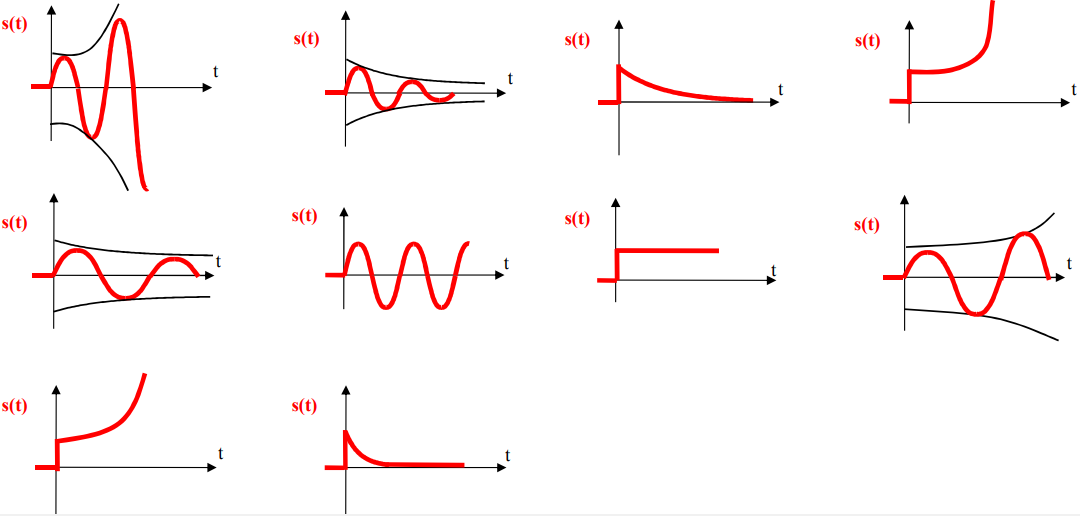
\includegraphics[width=.9\linewidth]{images/Sujet/images/fig_01}
}%figues de la page de garde


\def\xxpied{%
Cycle 01 -- Modéliser le comportement des systèmes multiphysiques\\
\xxactivite%
}

\setcounter{secnumdepth}{5}
%---------------------------------------------------------------------------

\usepackage{pgfplots}
\begin{document}
%\defimages{images}
%\chapterimage{png/Fond_Cin}
\pagestyle{empty}


%%%%%%%% PAGE DE GARDE COURS
\ifcours
% ==== BANDEAU DES TITRES ==== 
\begin{tikzpicture}[remember picture,overlay]
\node at (current page.north west)
{\begin{tikzpicture}[remember picture,overlay]
\node[anchor=north west,inner sep=0pt] at (0,0) {\includegraphics[width=\paperwidth]{\thechapterimage}};
\draw[anchor=west] (-2cm,-8cm) node [line width=2pt,rounded corners=15pt,draw=ocre,fill=white,fill opacity=0.6,inner sep=40pt]{\strut\makebox[22cm]{}};
\draw[anchor=west] (1cm,-8cm) node {\huge\sffamily\bfseries\color{black} %
\begin{minipage}{1cm}
\rotatebox{90}{\LARGE\sffamily\textsc{\color{ocre}\textbf{\xxnumpartie}}}
\end{minipage} \hfill
\begin{minipage}[c]{14cm}
\begin{titrepartie}
\begin{flushright}
\renewcommand{\baselinestretch}{1.1} 
\Large\sffamily\textsc{\textbf{\xxpartie}}
\renewcommand{\baselinestretch}{1} 
\end{flushright}
\end{titrepartie}
\end{minipage} \hfill
\begin{minipage}[c]{3.5cm}
{\large\sffamily\textsc{\textbf{\color{ocre} \discipline}}}
\end{minipage} 
 };
\end{tikzpicture}};
\end{tikzpicture}
% ==== FIN BANDEAU DES TITRES ==== 


% ==== ONGLET 
\begin{tikzpicture}[overlay]
\node[shape=rectangle, 
      rounded corners = .25 cm,
	  draw= ocre,
	  line width=2pt, 
	  fill = ocre!10,
	  minimum width  = 2.5cm,
	  minimum height = 3cm,] at (18.3cm,0) {};
\node at (17.7cm,0) {\rotatebox{90}{\textbf{\Large\color{ocre}{\classe}}}};
%{};
\end{tikzpicture}
% ==== FIN ONGLET 


\vspace{3.5cm}

\begin{tikzpicture}[remember picture,overlay]
\draw[anchor=west] (-2cm,-6cm) node {\huge\sffamily\bfseries\color{black} %
\begin{minipage}{2cm}
\begin{center}
\LARGE\sffamily\textsc{\color{ocre}\textbf{\xxactivite}}
\end{center}
\end{minipage} \hfill
\begin{minipage}[c]{15cm}
\begin{titrechapitre}
\renewcommand{\baselinestretch}{1.1} 
\Large\sffamily\textsc{\textbf{\xxnumchapitre}}

\Large\sffamily\textsc{\textbf{\xxchapitre}}
\vspace{.5cm}

\renewcommand{\baselinestretch}{1} 
\normalsize\normalfont
\xxcompetences
\end{titrechapitre}
\end{minipage}  };
\end{tikzpicture}
\vfill

\begin{flushright}
\begin{minipage}[c]{.3\linewidth}
\begin{center}
\xxfigures
\end{center}
\end{minipage}\hfill
\begin{minipage}[c]{.6\linewidth}
\startcontents
%\printcontents{}{1}{}
\printcontents{}{1}{}
\end{minipage}
\end{flushright}

\begin{tikzpicture}[remember picture,overlay]
\draw[anchor=west] (4.5cm,-.7cm) node {
\begin{minipage}[c]{.2\linewidth}
\begin{flushright}

\includegraphics[width=2cm]{logoCC}
\end{flushright}
\end{minipage}
\begin{minipage}[c]{.2\linewidth}
\textsl{\xxauteur} \\
\textsl{\classe}
\end{minipage}
 };
\end{tikzpicture}

\newpage
\pagestyle{fancy}

%\newpage
%\pagestyle{fancy}

\else
\fi
%% FIN PAGE DE GARDE DES COURS

%%%%%%%% PAGE DE GARDE TD
\iftd
%\begin{tikzpicture}[remember picture,overlay]
%\node at (current page.north west)
%{\begin{tikzpicture}[remember picture,overlay]
%\draw[anchor=west] (-2cm,-3.25cm) node [line width=2pt,rounded corners=15pt,draw=ocre,fill=white,fill opacity=0.6,inner sep=40pt]{\strut\makebox[22cm]{}};
%\draw[anchor=west] (1cm,-3.25cm) node {\huge\sffamily\bfseries\color{black} %
%\begin{minipage}{1cm}
%\rotatebox{90}{\LARGE\sffamily\textsc{\color{ocre}\textbf{\xxnumpartie}}}
%\end{minipage} \hfill
%\begin{minipage}[c]{13.5cm}
%\begin{titrepartie}
%\begin{flushright}
%\renewcommand{\baselinestretch}{1.1} 
%\Large\sffamily\textsc{\textbf{\xxpartie}}
%\renewcommand{\baselinestretch}{1} 
%\end{flushright}
%\end{titrepartie}
%\end{minipage} \hfill
%\begin{minipage}[c]{3.5cm}
%{\large\sffamily\textsc{\textbf{\color{ocre} \discipline}}}
%\end{minipage} 
% };
%\end{tikzpicture}};
%\end{tikzpicture}

%%%%%%%%%% PAGE DE GARDE TD %%%%%%%%%%%%%%%
%\begin{tikzpicture}[overlay]
%\node[shape=rectangle, 
%      rounded corners = .25 cm,
%	  draw= ocre,
%	  line width=2pt, 
%	  fill = ocre!10,
%	  minimum width  = 2.5cm,
%	  minimum height = 2.5cm,] at (18.5cm,0) {};
%\node at (17.7cm,0) {\rotatebox{90}{\textbf{\Large\color{ocre}{\classe}}}};
%%{};
%\end{tikzpicture}

% PARTIE ET CHAPITRE
%\begin{tikzpicture}[remember picture,overlay]
%\draw[anchor=west] (-1cm,-2.1cm) node {\large\sffamily\bfseries\color{black} %
%\begin{minipage}[c]{15cm}
%\begin{flushleft}
%\xxnumchapitre \\
%\xxchapitre
%\end{flushleft}
%\end{minipage}  };
%\end{tikzpicture}

% BANDEAU EXO
\iflivret % SI LIVRET
\begin{tikzpicture}[remember picture,overlay]
\draw[anchor=west] (-2cm,-3.3cm) node {\huge\sffamily\bfseries\color{black} %
\begin{minipage}{5cm}
\begin{center}
\LARGE\sffamily\color{ocre}\textbf{\textsc{\xxactivite}}

\begin{center}
\xxfigures
\end{center}

\end{center}
\end{minipage} \hfill
\begin{minipage}[c]{12cm}
\begin{titrechapitre}
\renewcommand{\baselinestretch}{1.1} 
\large\sffamily\textbf{\textsc{\xxtitreexo}}

\small\sffamily{\textbf{\textit{\color{black!70}\xxsourceexo}}}
\vspace{.5cm}

\renewcommand{\baselinestretch}{1} 
\normalsize\normalfont
\xxcompetences
\end{titrechapitre}
\end{minipage}};
\end{tikzpicture}
\else % ELSE LIVRET
\begin{tikzpicture}[remember picture,overlay]
\draw[anchor=west] (-2cm,-4.3cm) node {\huge\sffamily\bfseries\color{black} %
\begin{minipage}{5cm}
\begin{center}
\LARGE\sffamily\color{ocre}\textbf{\textsc{\xxactivite}}

\begin{center}
\xxfigures
\end{center}

\end{center}
\end{minipage} \hfill
\begin{minipage}[c]{12cm}
\begin{titrechapitre}
\renewcommand{\baselinestretch}{1.1} 
\large\sffamily\textbf{\textsc{\xxtitreexo}}

\small\sffamily{\textbf{\textit{\color{black!70}\xxsourceexo}}}
\vspace{.5cm}

\renewcommand{\baselinestretch}{1} 
\normalsize\normalfont
\xxcompetences
\end{titrechapitre}
\end{minipage}};
\end{tikzpicture}

\fi

\else   % FIN IF TD
\fi


%%%%%%%% PAGE DE GARDE FICHE
\iffiche
\begin{tikzpicture}[remember picture,overlay]
\node at (current page.north west)
{\begin{tikzpicture}[remember picture,overlay]
\draw[anchor=west] (-2cm,-3.25cm) node [line width=2pt,rounded corners=15pt,draw=ocre,fill=white,fill opacity=0.6,inner sep=40pt]{\strut\makebox[22cm]{}};
\draw[anchor=west] (1cm,-3.25cm) node {\huge\sffamily\bfseries\color{black} %
\begin{minipage}{1cm}
\rotatebox{90}{\LARGE\sffamily\textsc{\color{ocre}\textbf{\xxnumpartie}}}
\end{minipage} \hfill
\begin{minipage}[c]{14cm}
\begin{titrepartie}
\begin{flushright}
\renewcommand{\baselinestretch}{1.1} 
\large\sffamily\textsc{\textbf{\xxpartie} \\} 

\vspace{.2cm}

\normalsize\sffamily\textsc{\textbf{\xxnumchapitre -- \xxchapitre}}
\renewcommand{\baselinestretch}{1} 
\end{flushright}
\end{titrepartie}
\end{minipage} \hfill
\begin{minipage}[c]{3.5cm}
{\large\sffamily\textsc{\textbf{\color{ocre} \discipline}}}
\end{minipage} 
 };
\end{tikzpicture}};
\end{tikzpicture}

\iflivret
\begin{tikzpicture}[overlay]
\node[shape=rectangle, 
      rounded corners = .25 cm,
	  draw= ocre,
	  line width=2pt, 
	  fill = ocre!10,
	  minimum width  = 2.5cm,
	  minimum height = 2.5cm,] at (18.5cm,1.1cm) {};
\node at (17.9cm,1.1cm) {\rotatebox{90}{\textsf{\textbf{\large\color{ocre}{\classe}}}}};
%{};
\end{tikzpicture}
\else
\begin{tikzpicture}[overlay]
\node[shape=rectangle, 
      rounded corners = .25 cm,
	  draw= ocre,
	  line width=2pt, 
	  fill = ocre!10,
	  minimum width  = 2.5cm,
%	  minimum height = 2.5cm,] at (18.5cm,1.1cm) {};
	  minimum height = 2.5cm,] at (18.5cm,0cm) {};
\node at (18.5cm,0cm) {\rotatebox{90}{\textsf{\textbf{\large\color{ocre}{\classe}}}}};
%{};
\end{tikzpicture}

\fi

\else
\fi



\vspace{7cm}
\pagestyle{fancy}
\thispagestyle{plain}

\def\columnseprulecolor{\color{ocre}}
\setlength{\columnseprule}{0.4pt} 

%\defimages2{images}

%\begin{multicols}{2}
\section{Micromanipulateur compact pour la chirurgie endoscopique ($\text{MC}^2\text{E}$)}
\subsection{Présentation générale}
L’objet de cette étude est un robot appelé $\text{MC}^2\text{E}$ utilisé en chirurgie endoscopique. Ce type de
robots médico-chirurgicaux est équipé de capteurs (caméra, capteur d’efforts…) permettant de maîtriser
les interactions avec des environnements souvent déformables et difficilement modélisables comme le
corps humain.

\begin{center}
\begin{minipage}[c]{.1\linewidth}
\begin{center}
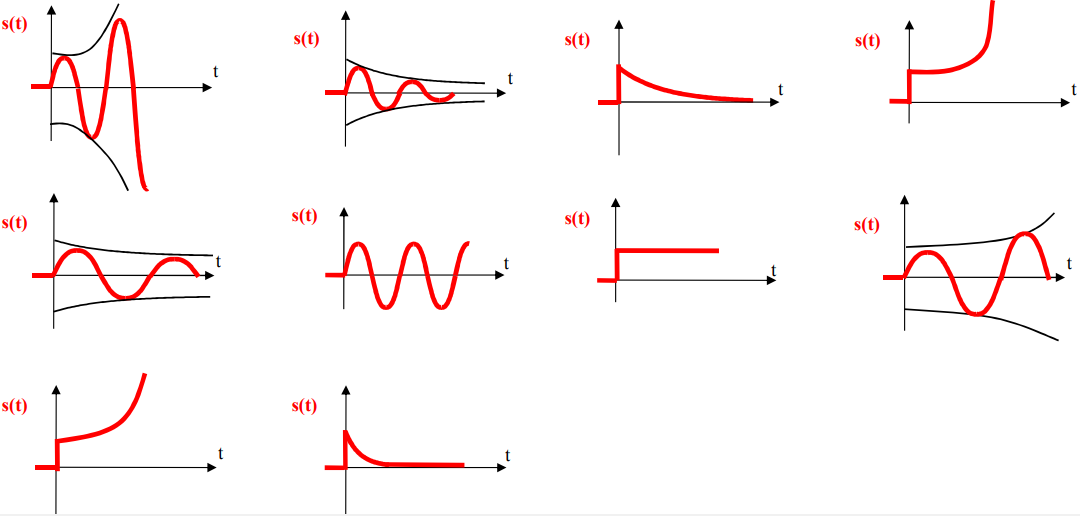
\includegraphics[height=4cm]{images/Sujet/images/fig_01}
\end{center}
\end{minipage} \hfill
\begin{minipage}[c]{.65\linewidth}
\begin{center}
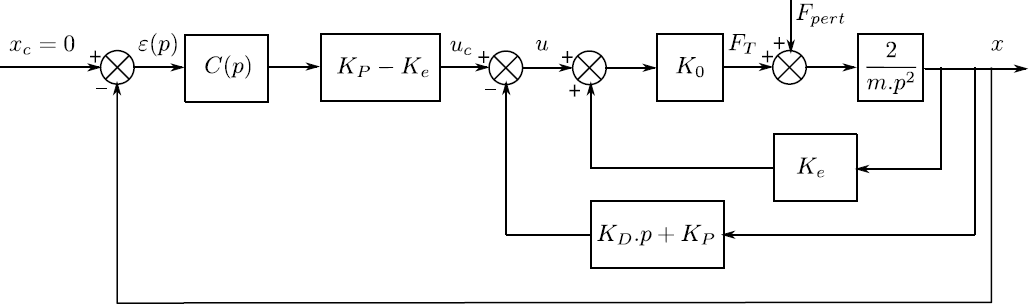
\includegraphics[height=3.5cm]{images/Sujet/images/fig_02}
%Figure 1 : Modèle de la commande en effort
\end{center}
\end{minipage}
\end{center}

Le mode opératoire se décompose en quatre phases :
\begin{itemize}
\item phase 1 : après avoir introduit le trocart, l’abdomen du patient est gonflé avec du $\text{CO}_2$. Celui-ci se montrera alors aussi stable et rigide que possible pour la réussite de l’opération ;
\item phase 2 : le $\text{MC}^2\text{E}$ est positionné sur l’abdomen du patient. Celui-ci est maintenu en position grâce à des sangles. Les trois axes en rotation sont alors asservis en position constante ;
\item phase 3 : la pince est introduite dans le trocart au travers d’un guide (étanche). Une phase de calibration du robot utile à la compensation de pesanteur analysée par la suite, démarre ;
\item phase 4 : le chirurgien amène la pince du $\text{MC}^2\text{E}$ qui doit tirer la vésicule lors de l’opération. 
\end{itemize}
L’axe en translation du $\text{MC}^2\text{E}$ entre alors en fonctionnement : il est asservi en effort constant pour tirer (ou pousser) la vésicule au fur et à mesure que le chirurgien utilise son bistouri pour détacher la vésicule du foie. La figure suivante décrit les principales exigences auxquelles est soumis le $\text{MC}^2\text{E}$.

\begin{center}
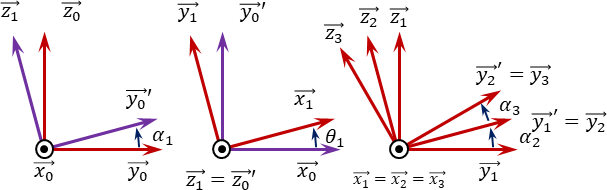
\includegraphics[width=\linewidth]{images/Sujet/images/fig_05}
%Figure 1 : Modèle de la commande en effort
\end{center}

%L’objectif de ce sujet est d’analyser, de comprendre et de justifier les choix structurels faits par les
%ingénieurs. Pour cela, on se basera sur la démarche de l’ingénieur :
%\begin{itemize}
%\item les exigences et/ou performances souhaitées sont spécifiées tout au long du sujet;
%\item des modèles et résultats analytiques ou simulés sont mis en place;
%\item des résultats expérimentaux sont proposés.
%\end{itemize}
%À chaque fois, on cherchera à quantifier les écarts entre les différents résultats obtenus par simulation et/ou
%expérimentation et les exigences et/ou performances souhaitées. Les réponses apportées aux questions
%devront donc être rédigées dans cet esprit.

\subsection{Validation des performances de l’asservissement d’effort}
On s’intéresse ici à la phase 4. Lors de l’opération envisagée, il est nécessaire de maintenir un effort
constant au bout de la pince (4). Pour cela, on réalise un asservissement d’effort de l’axe en translation que
l’on se propose d’étudier.
Le système est alimenté par un transformateur alternatif/continu. Un variateur permet de piloter le moteur
M4. Une interface de communication entrée/sortie permet de coder les consignes d’effort et acquérir des
grandeurs physiques. D’autre part, elle communique à la chaîne d’énergie, après traitement, des ordres
définis par un calculateur.
La description par diagramme partiel de définition de blocs de l’axe en translation est donnée ci-dessous. %Des modèles géométriques de cet axe sont donnés en annexe 5.


\begin{center}
%\begin{minipage}[c]{.45\linewidth}
\begin{center}
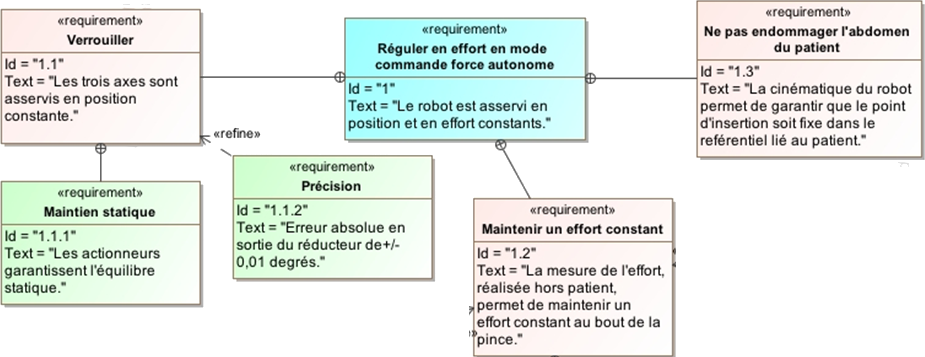
\includegraphics[height=9cm]{images/Sujet/images/fig_03}
\end{center}
%\end{minipage} \hfill
%\begin{minipage}[c]{.45\linewidth}
%\begin{center}
%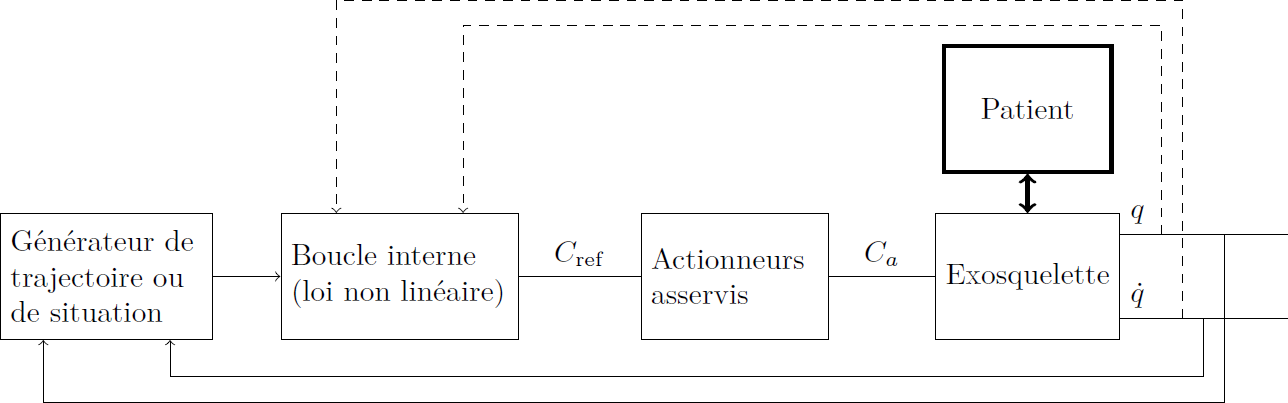
\includegraphics[height=4cm]{images/Sujet/images/fig_04}
%%Figure 1 : Modèle de la commande en effort
%\end{center}
%\end{minipage}
\end{center}

\subparagraph{}
\textit{Compléter le schéma représentant les chaînes d’énergie et d’information de cette chaîne
fonctionnelle asservie en indiquant le nom des composants réalisant chacune des fonctions.}

%
%
%Lors de l’opération, il est essentiel de contrôler et réguler l’effort appliqué sur l’organe et donc
%indirectement l’effort fourni par le moteur M4. Le schéma-blocs fonctionnel retenu pour la structure
%d’asservissement est donné figure 1. 
%
%\begin{center}
%%\includegraphics[width=\linewidth]{images/Sujet/images/}
%Figure 1 : Modèle de la commande en effort
%\end{center}
%
%A un effort de consigne va correspondre un effort appliqué sur l’organe
%pour l’extraire. C’est ce même effort qui est mesuré par le capteur
%d’effort. Celui-ci va alors générer un couple rapporté sur l’arbre du
%moteur M4.
%On souhaite ici s’intéresser à la structure de commande retenue pour
%cette boucle d’asservissement. Les interactions avec l’organe étant par
%définition inconnues et complexes, on va régler le calculateur en se
%basant sur un montage d’essai mettant en interaction la pince (4) avec
%un ressort simulant la vésicule biliaire (raideur du ressort similaire à la
%raideur de la vésicule).
%
%Le schéma-blocs fonctionnel retenu pour cette étude est donc le
%suivant :
%
%\begin{center}
%%\includegraphics[width=\linewidth]{images/Sujet/images/}
%Figure 2 : Modèle de la commande en effort
%\end{center}


\subsubsection*{Modèle de connaissance de l'asservissement}

\begin{obj}
Modéliser l’asservissement en effort.
\end{obj}

L’équation de mouvement est définie par l’équation différentielle suivante : 
$J\dfrac{\text{d}^2\theta_m(t)}{\text{d}t^2}=C_m(t)-C_e(t)$  avec :
\begin{itemize}
\item $J$, inertie équivalente à l’ensemble en mouvement, ramenée sur l’arbre moteur;
\item $C_e(t)$, couple regroupant l’ensemble des couples extérieurs ramenés à l’arbre moteur, notamment fonction de la raideur du ressort.
\end{itemize}


On notera $\theta_m(p)$, $\Omega_m(p)$, $C_m(p)$ et $C_e(p)$ les transformées de Laplace des grandeurs de l’équation de mouvement.
On pose $C_e(t)=K_{C\theta}\theta_m(t)$ où  $K_{C\theta}$ est une constante positive. On a de plus $\dfrac{\text{d}\theta_m(t)}{\text{d}t}=\omega_m(t)$. La régulation se met alors sous la forme du schéma-blocs à retour unitaire simplifié que l’on
admettra :

\begin{center}
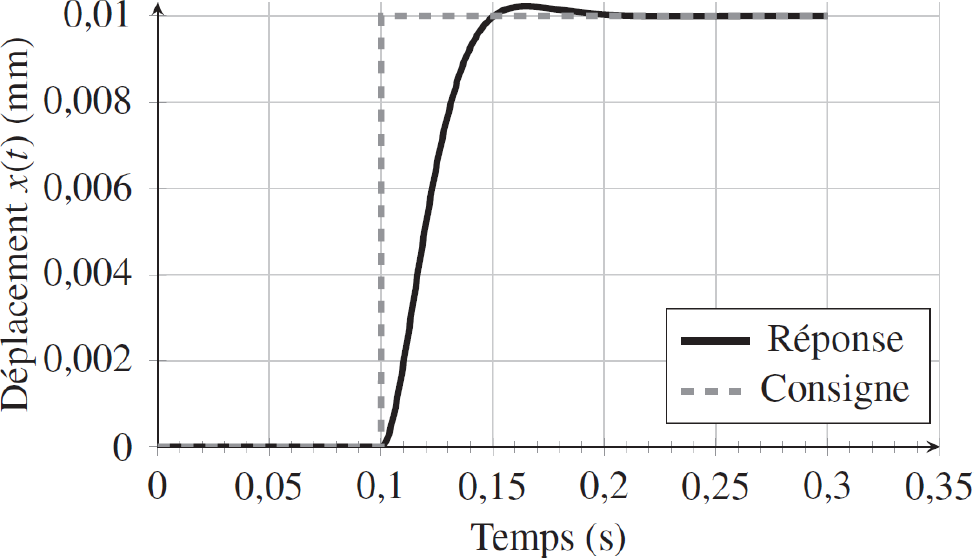
\includegraphics[width=.8\linewidth]{images/Sujet/images/fig_06}

\textit{Modèle simplifié du montage du capteur d’effort.}
\end{center}
%\end{multicols}

Avec :
\begin{itemize}
\item $C_e(p)$, couple de sortie mesuré par le capteur d’effort situé sur le $\text{MC}^2\text{E}$ ;
\item $C_c(p)$, couple de consigne ;
\item $C_m(p)$, couple moteur ;
\item $H_{\text{cor}}(p)$, fonction de transfert du correcteur.
\end{itemize}
Dans un premier temps, on prendra $H_{\text{cor}}(p)=1$.

\subparagraph{}
\textit{Déterminer les expressions des fonctions de transfert $H_1(p)$, $H_2(p)$ et $H_3(p)$.}
\ifprof
\begin{corrige}
\end{corrige}
\else
\fi

\subparagraph{}
\textit{Donner l’expression de la fonction de transfert en boucle fermée $H_{BF}(p)$ de l’asservissement
d’effort.}

\ifprof
\begin{corrige}
\end{corrige}
\else
\fi

\subparagraph{}
\textit{Quel sera le comportement de cet asservissement en réponse à un échelon d'amplitude $C_0$?
Conclure.}
\ifprof
\begin{corrige}
\end{corrige}
\else
\fi

\vspace{.25cm}

Pour remédier au problème ainsi mis en évidence, le concepteur a choisi de mettre en place une boucle
interne numérique, dite tachymétrique, de gain $B$. On s’intéresse ici à la définition analytique de $B$.
Le schéma-blocs modifié est donné figure suivante.


\begin{center}
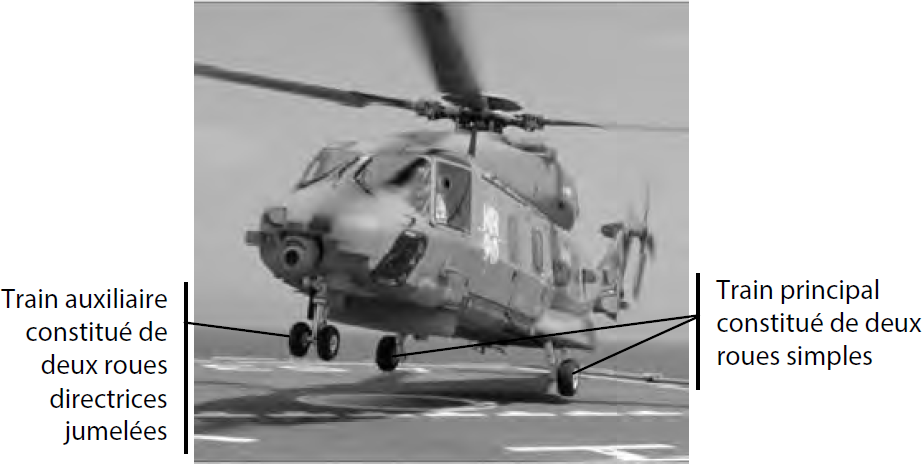
\includegraphics[width=.7\linewidth]{images/Sujet/images/fig_07}

\textit{Régulation avec retour tachymétrique}
\end{center}


On règle B de telle façon que, pour $H_{\text{cor}}(p)=1$, la fonction de transfert en boucle ouverte, notée $H_{\text{BO}}(p)$, puisse être mise sous la forme suivante : 
$H_{\text{BO}}(p)=\dfrac{1}{\left(1+\tau p\right)^2}$.



\subparagraph{}
\textit{Donner l’expression analytique du gain $B$, en fonction de $J$ et $K_{C\theta}$, permettant d’obtenir cette
forme de fonction de transfert. En déduire l’expression analytique de la constante de temps $\tau$.}
\ifprof
\begin{corrige}
\end{corrige}
\else
\fi

\vspace{.25cm}

Les exigences du cahier des charges sont données plus haut (exigences 1.2.2.1 à 1.2.2.4).

Afin de répondre à ces exigences, on choisit un correcteur proportionnel-intégral de gain $K_i$ et de constante de temps $T_i$. Le schéma-blocs de la régulation se met sous la forme de la figure qui suit.

\begin{center}
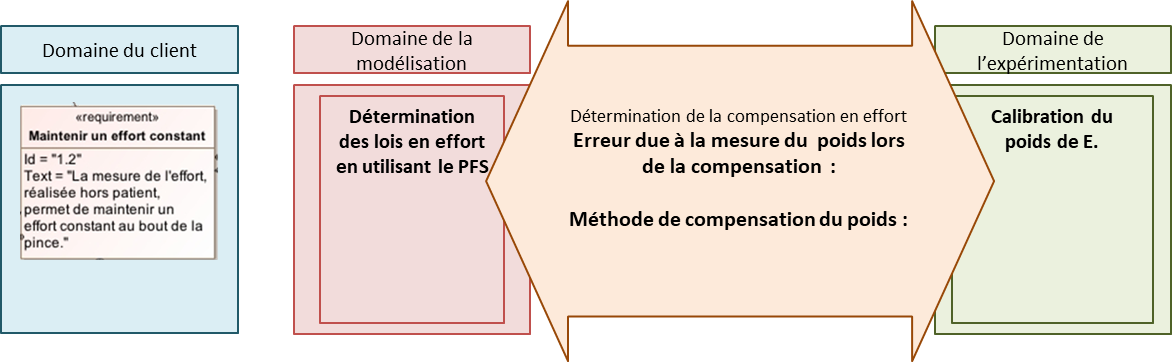
\includegraphics[width=.55\linewidth]{images/Sujet/images/fig_08}

\textit{Régulation avec correcteur PI.}
\end{center}


\subparagraph{}
\textit{Donner l’expression de l’erreur statique en réponse à un échelon d'amplitude $C_0$. Conclure vis-à-vis du cahier des charges.}
\ifprof
\begin{corrige}
\end{corrige}
\else
\fi

\vspace{.25cm}

On souhaite régler le correcteur pour que le système asservi ait une fonction de transfert en boucle fermée
d’ordre 2 de la forme :
$\dfrac{K_{\text{BF}}}{1+\dfrac{2\xi_{BF}}{\omega_{0\text{BF}}}p+\dfrac{p^2}{\omega_{0\text{BF}}^2}}$.


\subparagraph{}
\textit{Proposer une expression simple pour la constante de temps $T_i$.}
\ifprof
\begin{corrige}
\end{corrige}
\else
\fi

Sur le document réponse sont tracées les courbes de la réponse fréquentielle en boucle ouverte pour
$K_i=1$ et les réponses fréquentielles en boucle fermée pour différentes valeurs de $K_i$.


\subparagraph{}
\textit{En reportant les tracés nécessaires sur le document réponse et en utilisant les abaques 1 et 2 du
document réponse, proposer un choix de réglage pour $K_i$ permettant de vérifier toutes les
performances.}
\ifprof
\begin{corrige}
\end{corrige}
\else
\fi


\subparagraph{}
\textit{Remplir le tableau du document réponse et conclure sur la validation des critères de performance.
Tracer l’allure de la réponse temporelle à un échelon $C_{c0}$ en indiquant toutes les valeurs caractéristiques
nécessaires.}

\ifprof
\begin{corrige}

\end{corrige}
\else
\fi


\section{Direction automobile découplée}

\subsection{Mise en situation}

\noindent\begin{minipage}[c]{.67\linewidth}
\indent Le principe de la direction découplée est de substituer à la liaison mécanique entre le volant et les roues une architecture de type télémanipulateur à un degré de liberté qui consiste à coupler un robot maître manipulé par un opérateur, avec un robot esclave distant, qui effectue la tâche. 
\end{minipage}\hfill
\begin{minipage}[c]{.3\linewidth}
\begin{center}
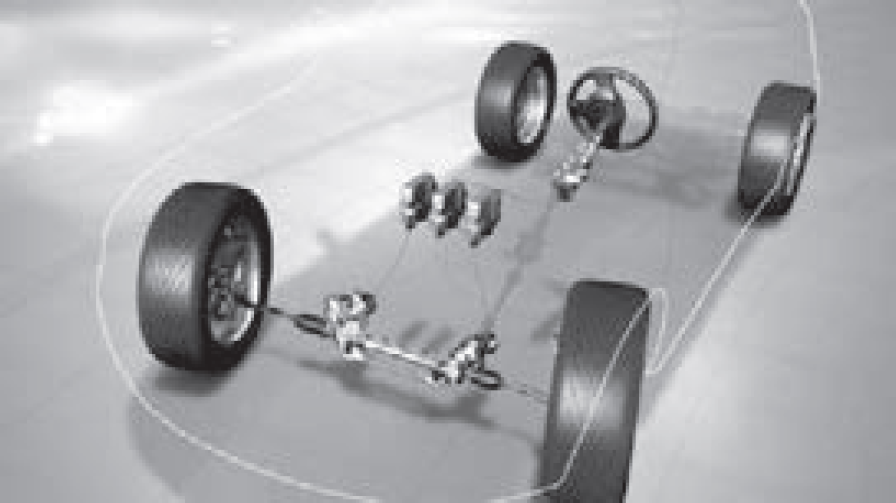
\includegraphics[width=4cm]{images/Sujet/images/img_01}
\end{center}
\end{minipage}

\subsection{Analyse et modélisation du système}
\begin{obj}
Cette partie a pour objectif d'analyser la structure et d'élaborer une modélisation du système
de direction découplée.
\end{obj}
Le diagramme de bloc interne précise la structure interne et les flux échangés
entre les différents composants de la direction découplée dont l'architecture est fournie par le
diagramme de définition de blocs.


\begin{center}
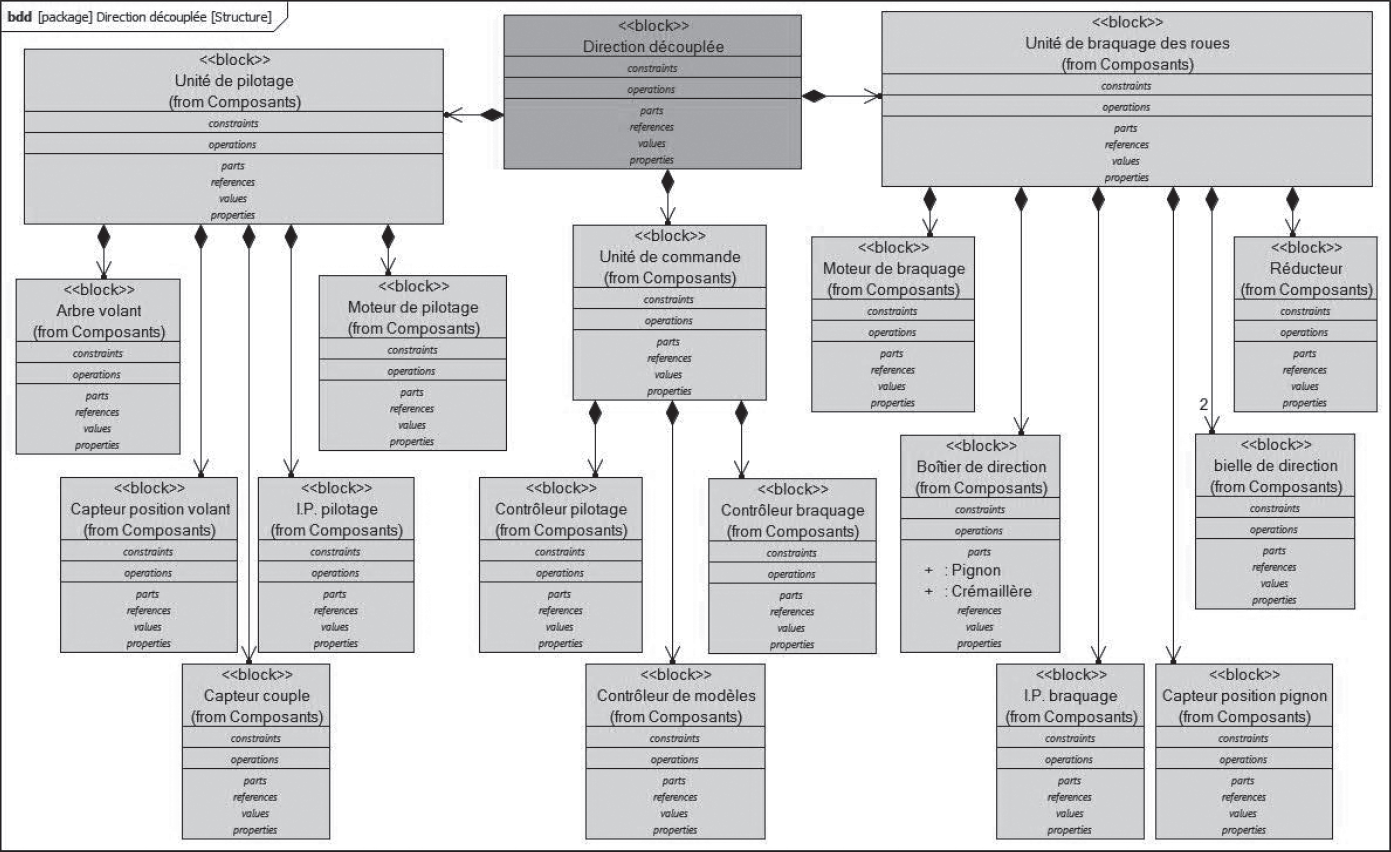
\includegraphics[width=\linewidth]{images/Sujet/images/fig_10}

\textit{Figure 1 -- Diagramme de blocs de la direction découplée.}
\end{center}
\begin{center}
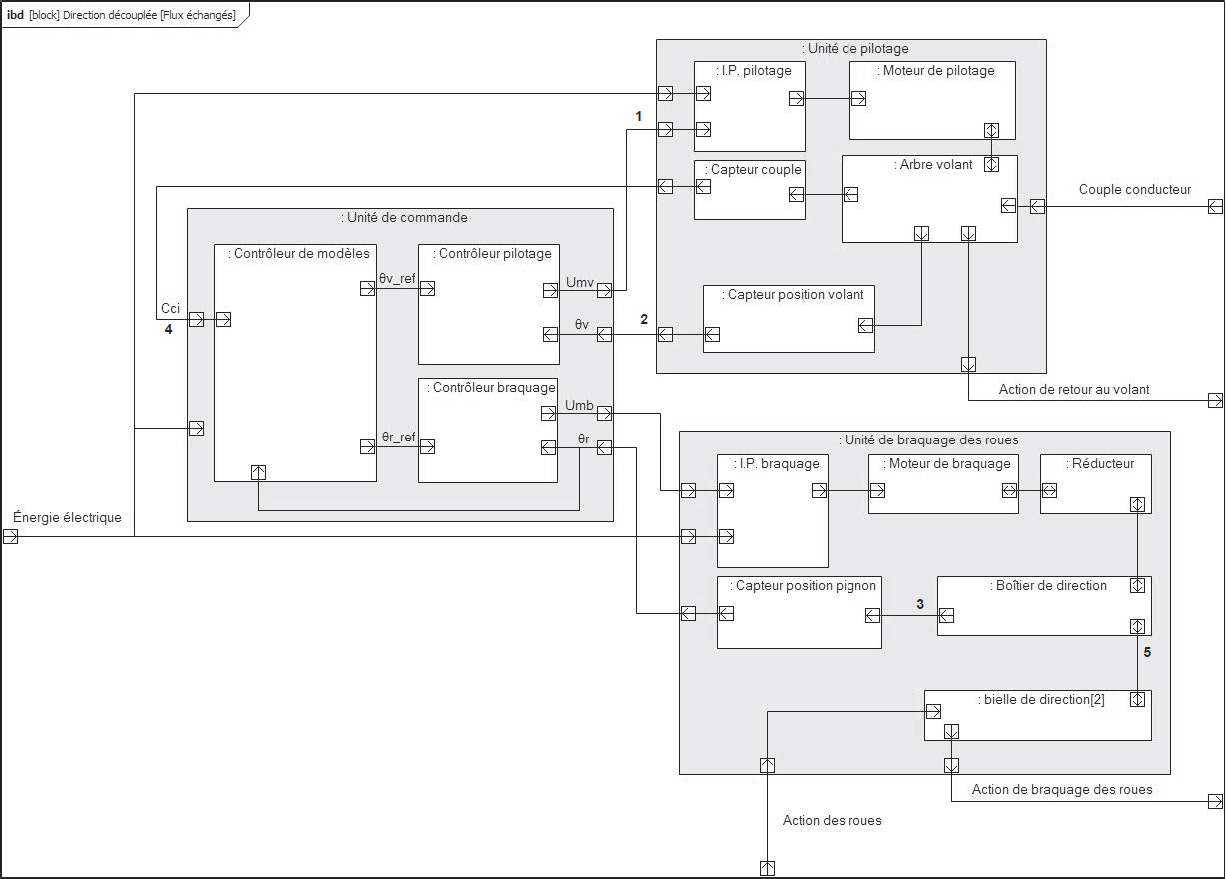
\includegraphics[width=\linewidth]{images/Sujet/images/fig_11}

\textit{Figure 2 -- Diagramme de blocs interne de la direction découplée.}
\end{center}

\subparagraph{}
\textit{Les unités de pilotage et de braquage comportent une interface de puissance (I.P.). Préciser la
fonction et le nom génériques de ce constituant au sein d'une chaîne fonctionnelle.}

\subparagraph{}
\textit{Préciser la nature (énergie ou information) des flux repérés 1, 2, 3, 4 et 5 sur le diagramme de bloc
interne.}
\ifprof
\begin{corrige}
\end{corrige}
\else
\fi

On donne dans le cahier réponses un schéma-blocs du modèle de la direction découplée.

%\subparagraph{}
%\textit{Les unités de pilotage et de braquage comportent une interface de puissance (I.P.). Préciser la
%fonction et le nom génériques de ce constituant au sein d'une chaîne fonctionnelle.}
%\ifprof
%\begin{corrige}
%\end{corrige}
%\else
%\fi



\subparagraph{}
\textit{Encadrer et nommer, sur le schéma-blocs du cahier réponses, les trois zones correspondant aux
unités de commande, de pilotage et de braquage définies sur le diagramme de blocs internes.}
\ifprof
\begin{corrige}
\end{corrige}
\else
\fi

\subsection{Modélisation et optimisation du comportement de l'unité de pilotage}

\begin{obj}
Cette partie a pour objectif de modéliser la structure de l'unité de pilotage, de simuler son
comportement et de corriger celui-ci afin d'obtenir les performances attendues et décrites
dans le cahier des charges.
\end{obj}

\subsubsection*{Cahier des charges}

\begin{center}
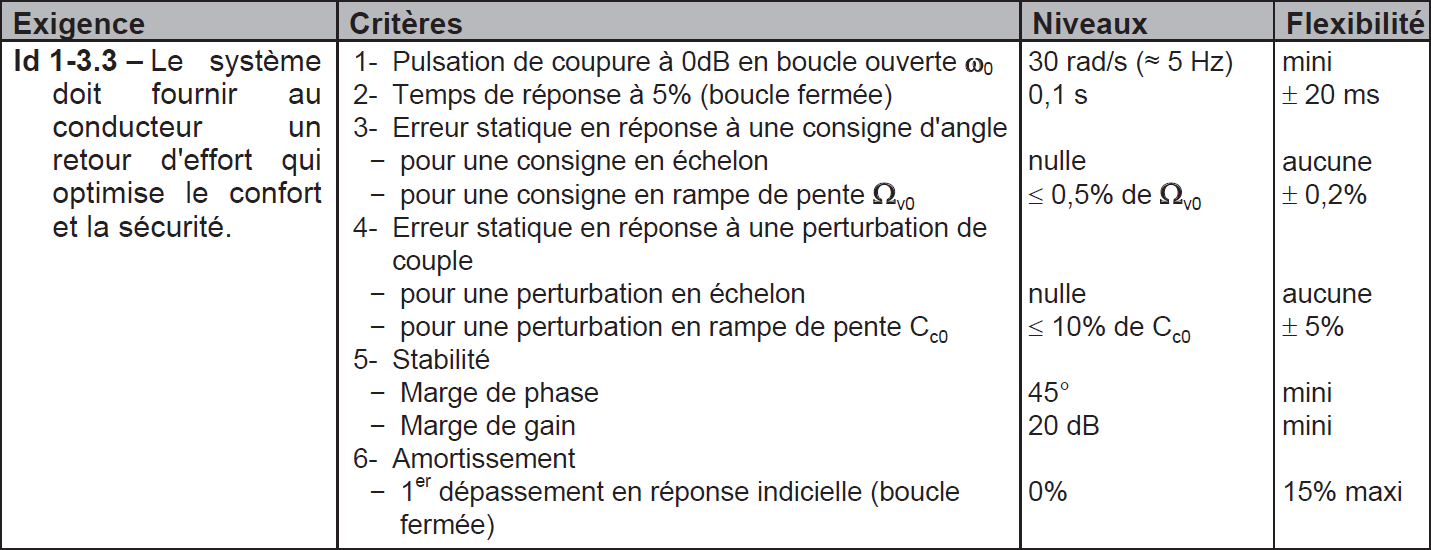
\includegraphics[width=\linewidth]{images/Sujet/images/fig_12}

%\textit{Diagramme de blocs interne de la direction découplée.}
\end{center}

On considère que l'évolution de référence du couple conducteur est une loi en trapèze donnée
figure suivante.


\begin{center}
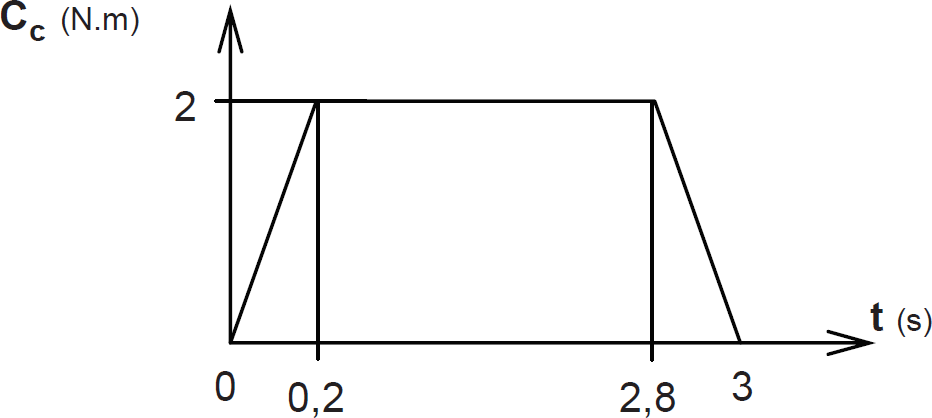
\includegraphics[width=.5\linewidth]{images/Sujet/images/fig_13}

\textit{Figure 3 -- Loi de référence en trapèze d'évolution du couple conducteur.}
\end{center}

La figure suivante donne une vue de cette unité sous la forme d'une maquette numérique à laquelle est
associé le schéma cinématique qui servira de base à l'étude mécanique.

\begin{center}
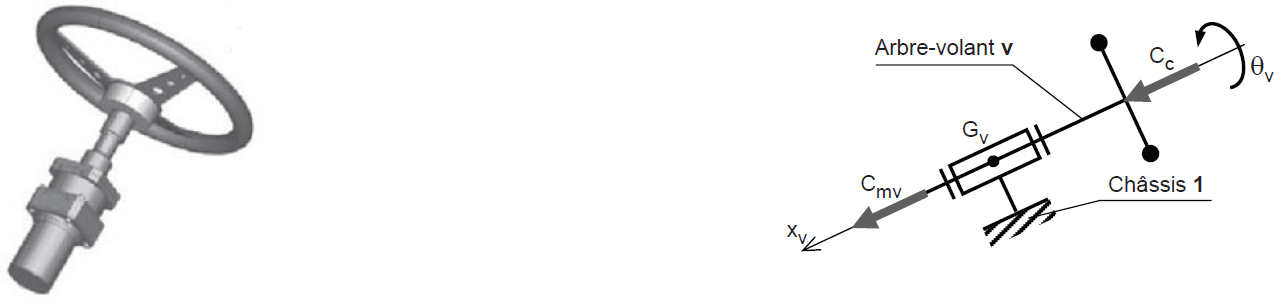
\includegraphics[width=\linewidth]{images/Sujet/images/fig_14}

\textit{Figure 4 -- Unité de pilotage (chaîne d'énergie) et schéma cinématique.}
\end{center}


L'unité de pilotage est constituée d'une chaîne d'énergie chargée de solliciter le volant par un
couple $C_{mv}\vect{x_v}$ qui résiste à l'action du conducteur $C_{c}\vect{x_v}$
quand celui-ci cherche à tourner le volant.

En effet, la simple dynamique du système mécanique de l'unité de pilotage ne donnerait pas au
conducteur la sensation de manier la direction d'une automobile. La composante $C_{mv}$ est donc élaborée
pour que la dynamique du volant en termes d'inertie et de raideur soit équivalente à celle d'une direction
conventionnelle optimisée selon le type de conduite visée.

La composante $C_{mv}$ est élaborée à partir de la consigne d'angle du volant $\theta_{v\_ref}$, transmise par le
générateur de consigne intégré au contrôleur de modèles, et de la composante $C_c$ du couple
conducteur.
Le modèle de la structure sous la forme d'un schéma-blocs décrivant le comportement asservi de cette
unité est donné figure suivante. On précise que la variable d'entrée est $\theta_{v\_ref}(p)$, que la variable de sortie est $\theta_{v}(p)$ et que la variable $C_c(p)$ est considérée comme une perturbation. Un signal de commande
$U_{mv}(p)$ pilote la motorisation.


\begin{center}
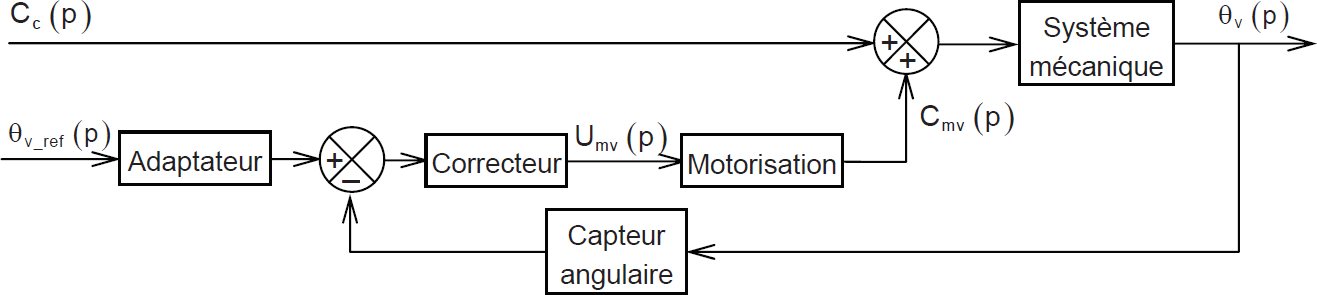
\includegraphics[width=\linewidth]{images/Sujet/images/fig_15}

\textit{Figure 5 -- Schéma-blocs de l'unité de pilotage.}
\end{center}

Un modèle acausal de cette structure dont certains composants ne sont pas reliés aux autres, est
donné sur le cahier réponses.

\subparagraph{}
\textit{Compléter ce modèle en traçant les liens manquants qui donneraient un modèle équivalent au
schéma-blocs précédent.}
\ifprof
\begin{corrige}
\end{corrige}
\else
\fi

\vspace{.25cm}
Le modèle cinématique utilisé pour la structure est celui donné en figure 4.

Notations :
\begin{itemize}
\item arbre-volant \textbf{v} : le solide constitué du rotor du moteur, de l'arbre volant et du volant ;
%\item Gv : centre d'inertie de l'arbre-volant v ;
%\item I(v,Gv) : opérateur d'inertie de v au point Gv ;
\item $J_v$ : le moment d'inertie de \textbf{v} autour de l'axe $\left( G_v,\vect{x_v}\right)$;
\item $f_v$ : le coefficient de frottement visqueux de la liaison pivot ;
\item $\theta_v(t)$ : l'angle de rotation de l'arbre-volant \textbf{v} par rapport au châssis 1 (noté $\theta_v(p)$ dans le domaine de Laplace);
\item $\omega_v(t)$ : la vitesse de rotation de l'arbre-volant \textbf{v} par rapport au châssis 1 (noté $\Omega_v(p)$ dans le
domaine de Laplace).
\end{itemize}

Le théorème du moment dynamique suivant l’axe $\left(G_v,\vect{x_v}\right)$ permet d’écrire :
$$
C_c(t)+C_{mv}(t)-f_v\dot{\theta_v}(t)=J_v\ddot{\theta_v}(t).
$$

On a par ailleurs $\dfrac{\text{d}\theta_v(t)}{\text{d} t}=\omega_v(t)$

\subparagraph{}
\textit{En supposant les conditions initiales nulles, donner la traduction du théorème du moment dynamique dans le
domaine de Laplace en fonction de $\Omega_v(p)$, $C_c(p)$ et $C_{mv}(p)$.  Exprimer alors la fonction de transfert $T_v(p)$ telle que 
$\Omega_v(p)=T_v(p)\left( C_c(p)+C_{mv}(p)\right)$ sous la forme $T_v(p)=\dfrac{g_v}{1+\tau_vp}$ dont on donnera l'expression de $g_v$ et $\tau_v$ en fonction de $f_v$ et $J_v$.}
\ifprof
\begin{corrige}
\end{corrige}
\else
\fi

\subsection{Analyse et optimisation du comportement de l'unité de pilotage}
Le schéma-blocs dont la structure est donnée figure 5 devient, pour l'étude du comportement, celui de
la figure 6 où le retour est unitaire. On note $\varepsilon_{\theta v}(t)$ l'écart entre la consigne et l'angle obtenu, et $\varepsilon_{c v}(t)$ le couple résultant des couples $C_c$ et $C_{mv}$.


\begin{center}
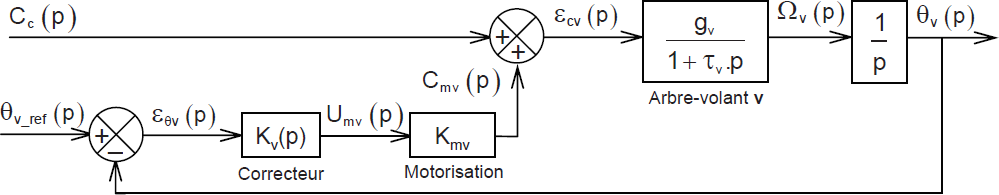
\includegraphics[width=\linewidth]{images/Sujet/images/fig_16}

\textit{Figure 6 -- Schéma-blocs de l'unité de pilotage.}
\end{center}

En considérant que la dynamique électromécanique du moteur seul est négligeable devant celle de
l'arbre-volant, on adopte pour la motorisation constituée du moteur à courant continu et de son
électronique de commande, comportant notamment une boucle de courant, un modèle sous la forme
d'un gain pur. On lui associe le gain $K_{mv}$.

Pour les applications numériques, on prendra les valeurs suivantes : 
$g_v = \SI{5}{rad.s^{-1}.N^{-1}.m^{-1}}$; $\tau_v=\SI{0,1}{s}$ et $K_{mv} = \SI{0,4}{N.m.V^{-1}}$.


\subsubsection*{Correction proportionnelle intégrale}
On choisit un correcteur proportionnel intégral (PI) tel que $K_v(p)=K_i\dfrac{1+\tau_i p}{\tau_i p}$ avec $\tau_i=\alpha \tau_v$.




\textbf{On considère pour cette question (15) uniquement que $C_c(p)=0$.}
\subparagraph{}
\textit{Exprimer la fonction de transfert en boucle ouverte $\text{FTBO}_{v1}(p)$ du système corrigé, avec le
correcteur PI, telle que $\theta_v(p)=\text{FTBO}_{v1}(p) \varepsilon_{\theta v}(p)$ sous la forme
$\text{FTBO}_{v1}(p)=K_{BOv1}\dfrac{1}{p^2}H(p)$ pour laquelle on précisera les expressions de $K_{BOv1}$ et de $H(p)$ de gain statique unitaire.}


\ifprof
\begin{corrige}
\end{corrige}
\else
\fi
\vspace{.25cm}

On admet que $\alpha$ doit être supérieur à 1 pour que le système puisse être stabilisé. On commence par choisir $\tau_i$ en prenant $\alpha=10$ et on cherche à optimiser $K_i$.

\subparagraph{}
\textit{Exprimer $\varepsilon_{\theta v}(p)$ en fonction de $\theta_{v\_ref}(p)$ et $C_c(p)$ et $\text{FTBO}_{v1}(p)$ (liste non exhaustive de paramètres).}

\ifprof
\begin{corrige}
\end{corrige}
\else
\fi


\subparagraph{}
\textit{Quelle doit être la valeur minimale de $K_i$ pour que les critères de précision soient satisfaits ? (On détaillera donc la valeur minimale que doit prendre $K_i$ pour les critères 3 et 4 de l'exigence 1-3.3.)}
\ifprof
\begin{corrige}
\end{corrige}
\else
\fi

On donne sur le cahier réponses le tracé du lieu de transfert de la $\text{FTBO}_{v1}(p)$ dans le plan de Bode,
pour $K_i = \SI{0,5}{V.rad^{-1}}$.


\subparagraph{}
\textit{Tracer sur le lieu de transfert de la $\text{FTBO}_{v1}(p)$ du cahier réponses, les diagrammes asymptotiques
dans le plan de Bode. On justifiera les valeurs particulières de pentes, de pulsations,
de gains et de phases.}
\ifprof
\begin{corrige}
\end{corrige}
\else
\fi

On choisit finalement $K_i=\SI{5}{V.rad^{-1}}$.
%
%On note :
%\begin{itemize}
%\item $\varphi(\omega)$ la phase de $H(p)$, soit $\arg[H(j\omega)]$ ;
%\item $\omega_{\ell}$ la plus grande pulsation qui vérifie $ \varphi(\omega=\omega_{\ell})=45\degres$.
%\end{itemize}
%On donne (figures suivantes) l'évolution de cette pulsation $\omega_{\ell}$ en fonction de $\alpha$ et un abaque qui représente la valeur maximale $\varphi_m$ de $\varphi(\omega)$ en fonction de $\alpha$.
%
%
%\subparagraph{}
%\textit{Peut-on obtenir la valeur minimale de la pulsation de coupure à $\SI{0}{dB}$ en boucle ouverte, $\omega_0$, fixée au cahier des charges en modifiant la valeur de $\alpha$ et/ou $K_i$ ? On pourra s'aider des abaques suivants pour justifier la réponse.}
%
%\ifprof
%\begin{corrige}
%\end{corrige}
%\else
%\fi
%
%
%
%\begin{center}
%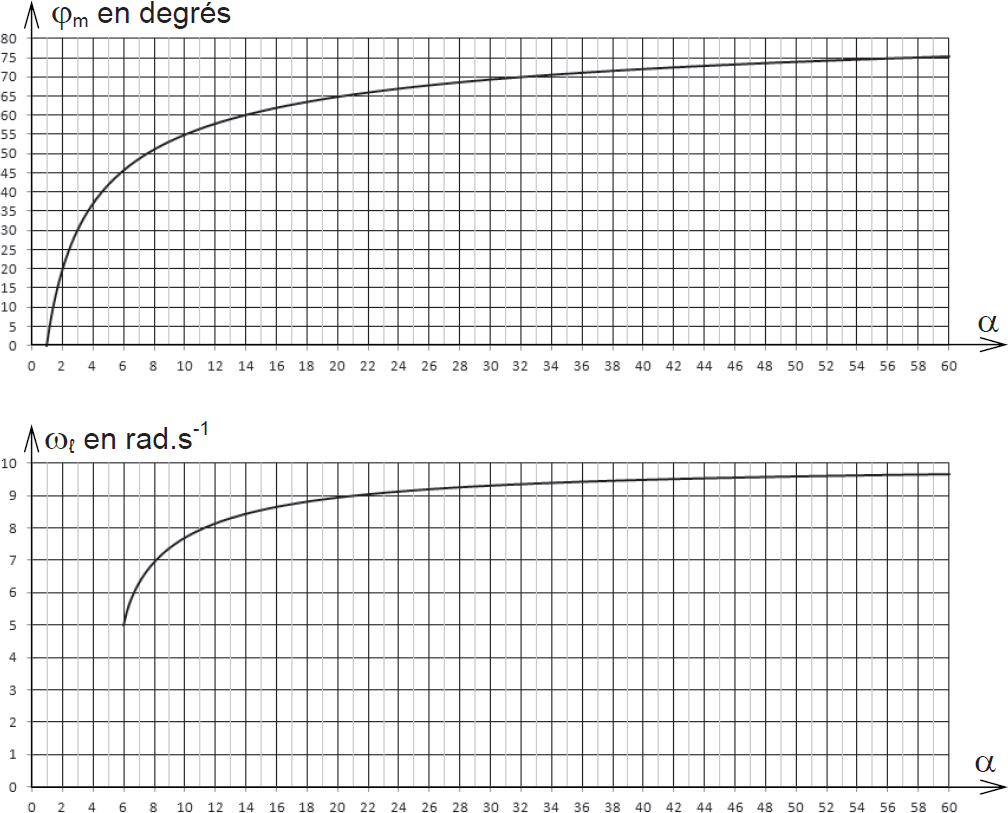
\includegraphics[width=\linewidth]{images/Sujet/images/fig_17}
%%B1
%\textit{Abaques de réglage de $H(p)$ en fréquentiel.}
%\end{center}
%
On donne figure suivante, en réponse à un échelon en boucle fermée, les abaques du temps de
réponse à 5\% et du 1\ier dépassement en \% de la valeur finale, en fonction de $K_i$ et pour $\alpha = 10$.


\begin{center}
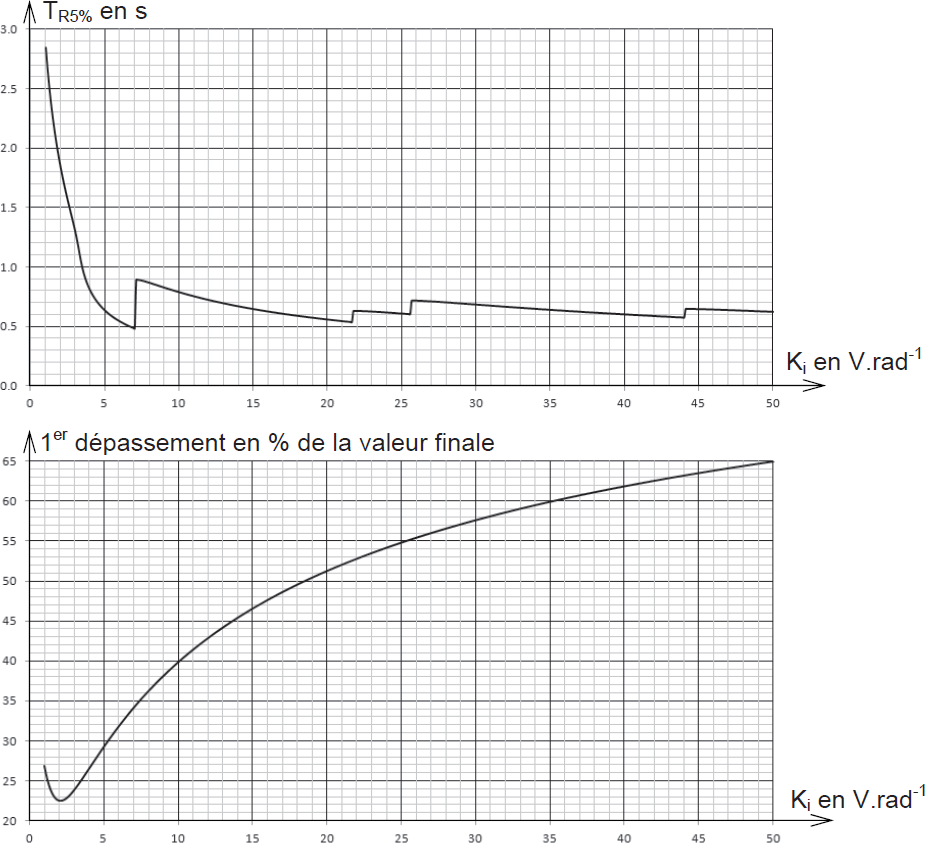
\includegraphics[width=.8\linewidth]{images/Sujet/images/fig_18}
%B2

\textit{Figure 7 --  Abaques de réglage en temporel de l'unité de pilotage corrigée.}
\end{center}


\subparagraph{}
\textit{Conclure sur les capacités de cette correction à satisfaire les critères de l'exigence Id 1-3.3 en
reprenant chaque critère.}
\ifprof
\begin{corrige}
\end{corrige}
\else
\fi



\subsubsection*{Correction proportionnelle intégrale et retour tachymétrique}

On ajoute à la correction précédente, une correction par retour tachymétrique tel que le décrit le
schéma-blocs suivant. On note $K_{rt}$ le gain statique du retour tachymétrique.


\begin{center}
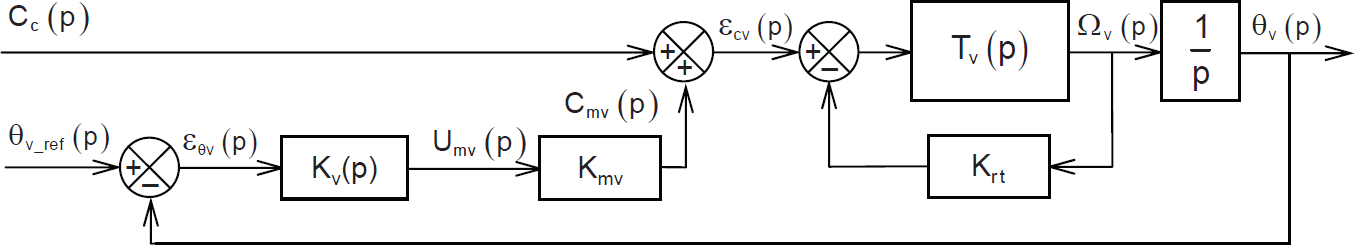
\includegraphics[width=\linewidth]{images/Sujet/images/fig_20}

\textit{Figure 8 -- Schéma-blocs de l'unité de pilotage avec retour tachymétrique.}
\end{center}



\subparagraph{}
\textit{Au vu des conclusions de la question précédente, donner des arguments qui précisent l'objectif
poursuivi par la mise en \oe{}uvre d'une telle correction.}
\ifprof
\begin{corrige}
\end{corrige}
\else
\fi


\subparagraph{}
\textit{Exprimer la fonction de transfert en boucle fermée $T_{vrt}(p)$ définie par $\Omega_v(p)=T_{vrt}(p)\varepsilon_{cv}(p)$ en fonction de $T_v (p)$ et $K_{rt}$. Mettre alors $T_{vrt}(p)$ sous la forme $T_{vrt}(p)=T_v(p)\beta\dfrac{1+\tau_v p}{1+\beta \tau_v p}$, pour laquelle, on précisera l'expression de $\beta$ en fonction de $K_{rt}$ et du gain statique $g_v$ défini précédemment.}
\ifprof
\begin{corrige}
\end{corrige}
\else
\fi


\subparagraph{}
\textit{Montrer que la nouvelle fonction de transfert en boucle ouverte $\text{FTBO}_{v2}(p)$, telle que
$\theta_v(p)=\text{FTBO}_{v2}(p)\varepsilon_{\theta v}(p)$, peut ainsi se mettre sous la forme $\text{FTBO}_{v2}(p)=K_{\text{BOv2}}\dfrac{1}{p^2}\dfrac{1+\alpha \tau_v p}{1+\beta \tau_v p}$,  pour laquelle on donnera l'expression de $K_{\text{BOv2}}$ en fonction de $K_{mv}$, $g_v$, $\tau_v$, $K_f$, $\alpha$ et $\beta$.}

\ifprof
\begin{corrige}
\end{corrige}
\else
\fi

\vspace{1cm}

\textit{Il resterait les mêmes calculs que précédemment à réaliser afin de vérifier si le cahier des charges est satisfait...}
%On donne sur le cahier réponses le tracé du lieu de transfert de la $\text{FTBO}_{v2}(p)$ dans le plan de Bode,
%pour $K_i = \SI{1,2}{V.rad^{-1}}$ (valeur évitant des calculs trop longs), réglé avec $\beta=1/ 6$ (non justifié) et pour $\alpha = 10$ (valeur choisie précédemment).
%


%
%\subparagraph{}
%\textit{Justifier que $\beta$ doit être inférieur à 1 pour que la correction par retour tachymétrique soit efficace vis-à-vis du critère de pulsation de coupure à \SI{0}{dB}.}
%\ifprof
%\begin{corrige}
%\end{corrige}
%\else
%\fi

%On donne, pour le système en boucle fermée et non perturbé (couple conducteur
%nul), les abaques du temps de réponse à 5\% et du premier dépassement en réponse à un échelon d'angle $\theta_{v\_\text{ref}}$, en fonction de la marge de phase du système, réglé avec $\beta=1/ 6$.
%
%\begin{center}
%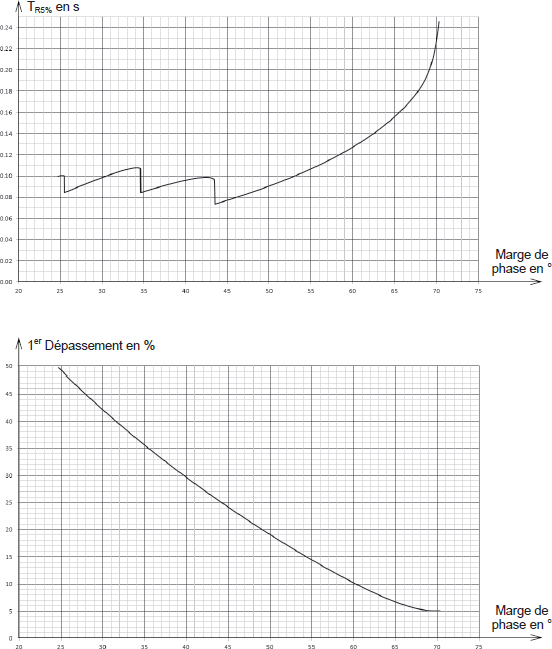
\includegraphics[width=\linewidth]{images/Sujet/images/fig_19}
%%B^''?
%\textit{Abaques de réglage en temporel de l'unité de pilotage corrigée avec retour tachymétrique.}
%\end{center}
%
%
%\subparagraph{}
%\textit{Faire une synthèse argumentée de la démarche proposée dans cette partie, pour optimiser le
%comportement de l'unité de pilotage.
%Conclure, en reprenant chaque critère de l'exigence Id 1-3.3, sur la satisfaction du cahier des
%charges.}
%\ifprof
%\begin{corrige}
%\end{corrige}
%\else
%\fi

%\subparagraph{}
%\textit{Avec le réglage établi par le modèle, quel phénomène pourrait endommager certains composants
%du système réel ?
%Quelle disposition technologique permettrait d'éviter ce phénomène ? Quelles en seraient les
%conséquences sur les performances du système ?}
%\ifprof
%\begin{corrige}
%\end{corrige}
%\else
%\fi
%
%\subparagraph{}
%\textit{}
%\ifprof
%\begin{corrige}
%\end{corrige}
%\else
%\fi
%
%\subparagraph{}
%\textit{}
%\ifprof
%\begin{corrige}
%\end{corrige}
%\else
%\fi



%%%%%%%%%%%%%%%%%%%%%%%%%%%%%%%%
%%%%%%%%%%%%%%%%%%%%%%%%%%%%%%%%
%%%%%%%%%%%%%%

\section{Robot endoscopique}% \footnote{D'après concours Banque PT.}]

\subsection{Analyser le besoin du robot endoscopique\\}
Les avancées technologiques dans le domaine de la chirurgie permettent actuellement
de réaliser des opérations de très grande complexité (chirurgie cardiaque,
digestive, urologique...) avec des avantages pour le patient qui proviennent de la limitation
des zones de dissection, ce qui réduit considérablement le traumatisme
opératoire.

La chirurgie endoscopique consiste à réaliser des opérations à
l’aide d’outils chirurgicaux de très petite taille, placés à l’extrémité
de tiges tubulaires tenues par le chirurgien. La partie inférieure des
tiges est insérée dans la zone à traiter, à travers trois petits orifices
réalisés dans le corps du patient (entre les côtes, par exemple, pour
une chirurgie cardiaque).
La chirurgie endoscopique robotisée utilise des robots à actionneurs
électriques pour positionner et commander les instruments.

Les trois robots appelés « robots esclaves » portent les instruments,
dont l’endoscope.
Le « robot esclave » étudié est constitué de 3 axes permettant de déplacer l’instrument
chirurgical positionné sur la plaque support en translation selon les trois directions
de l’espace X , Y et Z .

\begin{center}%[!ht]
%\centering
	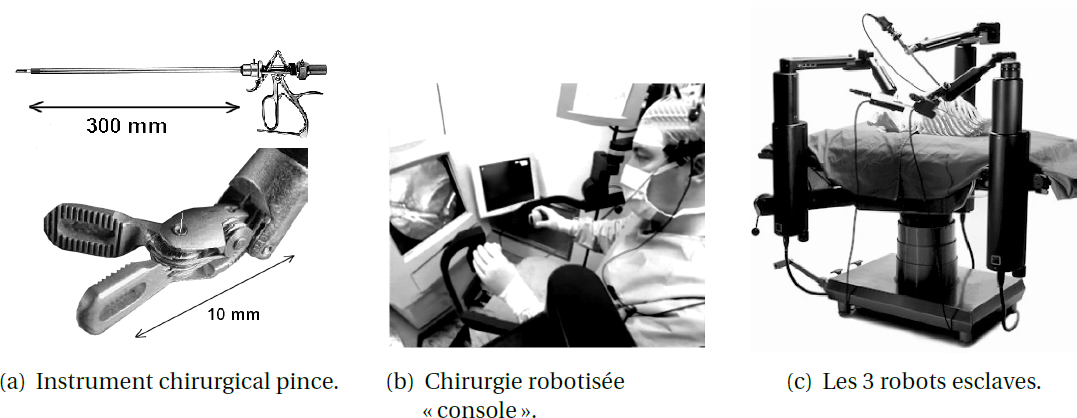
\includegraphics[width=\linewidth]{images/Sujet/images/img_02}
	%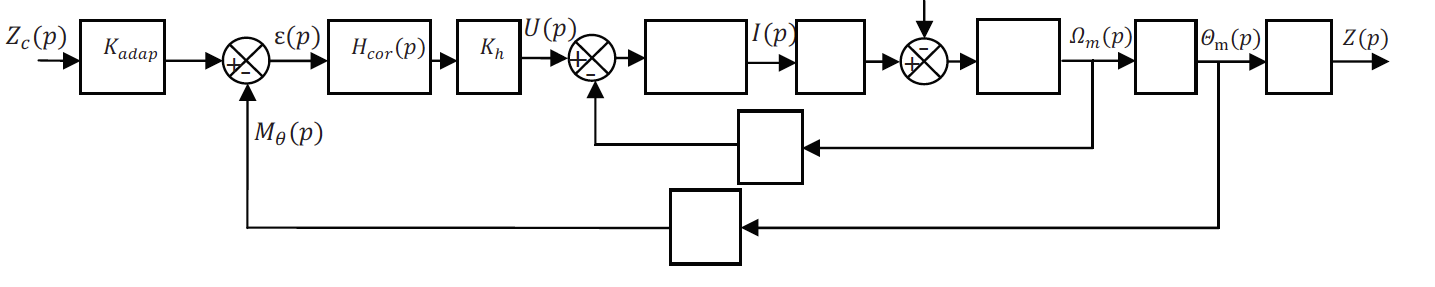
\includegraphics[width=.8\linewidth]{images2/schema_bloc}
	\textit{Présentation du matériel de téléchirurgie.}
%	\label{p04_robot_endo:fig1}}
\end{center}

 On considère à nouveau l'axe d'élévation du dispositif de commande de l'instrument chirurgical décrit par le schéma-blocs suivant.

\begin{center}%[!ht]
%\centering
	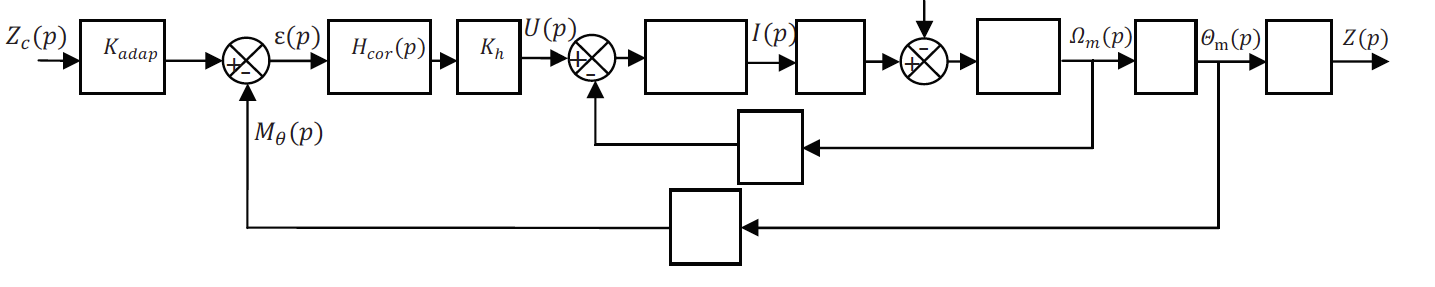
\includegraphics[width=\linewidth]{images2/schema_bloc}
	%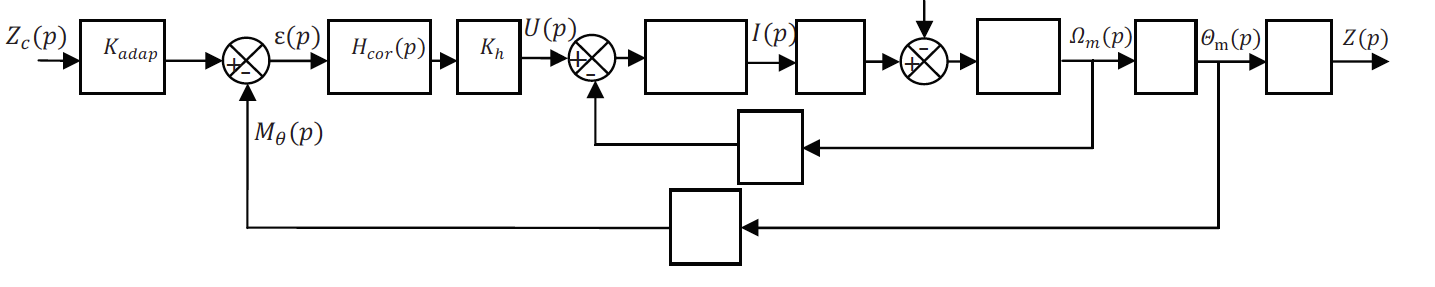
\includegraphics[width=.8\linewidth]{images2/schema_bloc}
	\textit{Schéma-blocs de l'axe d'élévation.}
%	\label{p04_robot_endo:fig1}}
\end{center}

La console permet de capter le déplacement de la main, de le coder, de le corriger éventuellement afin d'élaborer la consigne de position angulaire du moteur. La position angulaire est ensuite transformée en position linéaire de l'instrument par un mécanisme de transformation de mouvement à crémaillère.

\begin{obj}
Compte tenu de la chaîne cinématique et de l'asservissement mis en place, la raideur des transmetteurs peut jouer sur le critère de précision de l'axe. L'objectif de l'étude est de montrer par une étude fréquentielle que le système respecte le critère de bande passante du cahier des charges.
\end{obj}

Le cahier des charges est décrit par le diagramme des exigences suivant.


\begin{center}%[!htb]
\centering
%\includegraphics[width=.9\textwidth]{images2/C1.png}
%\includegraphics{images2/C1.pdf}

\includegraphics[width=\linewidth]{images2/Diagramme_exigences}

\textit{Diagramme des exigences partiel.}
%\label{p04_fig_exigences}
\end{center}

\subsection{Déterminer la fonction de transfert de l'asservissement de position angulaire}


\subsubsection*{Modéliser le comportement du moteur\\}
		
On cherche dans un premier temps à déterminer la fonction de transfert de l'asservissement de position angulaire. Une identification temporelle a permis de proposer un modèle du premier ordre pour l'ensemble moto-réducteur.  La fonction de transfert est alors la suivante : $M(p)=\frac{\num{0.44}}{1+\num{0.015} p}$.


Une identification fréquentielle du moto-réducteur est alors mise en place pour valider le modèle. On obtient les diagrammes de Bode suivant.

\begin{center}
\includegraphics[width=.6\linewidth]{images2/bode_1}

\textit{Identification fréquentielle du moto-réducteur.}
\end{center}

\subparagraph{}\textit{\label{p02_robot_endo:qdr2} Justifier au regard de la courbe que le modèle est pertinent dans une certaine bande de pulsations à préciser. Vérifier que les coefficients obtenus pour la fonction de transfert du moto-réducteur par l'identification temporelle sont cohérents avec ceux obtenus par identification fréquentielle.}

%\interenum{
%\begin{methode}
%Pour justifier un modèle à partir des diagrammes de Bode, il faut décrire les asymptotes sur les \textbf{deux} diagrammes et les comparer aux modèles élémentaires du premier et du second ordre.
%L'identification de paramètres se fait sur la valeur initiale de gain et à partir de pulsations pour des valeurs particulières du déphasage.
%\end{methode}




%\begin{center}%[!ht]
%%\centering
%\begin{tikzpicture}[xscale=16/10,yscale=1/40]
%\UnitedB
%\OrdBode{20}
%\semilog{0}{5}{-100}{0}
%\BodeAmp[cyan,thick]{0:5}{\SOAmp{0.436}{4.12}{568}}
%\end{tikzpicture}
%
%\begin{tikzpicture}[xscale=16/10,yscale=1/70]
%\UniteDegre
%\OrdBode{30}
%\semilog{0}{5}{-180}{0}
%\BodeArg[cyan,thick]{0:5}{\SOArg{0.436}{4.12}{568}}
%\end{tikzpicture}
%
%	%\includegraphics[width=.6\linewidth]{images2/identification_temp_moteur}
%	\textit{Identification fréquentielle du moto-réducteur.}
%	%\label{p04_robot_endo:fig3}
%	%\textcolor{red}{ DI *** A TRACE DIAG BODE de $\frac{0.436}{1+14,5.10^{-3}.p+3,1.10^{-6}.p^2}$}
%	
%\end{center}
%
%\vspace{-1em}
\subsubsection*{Modéliser l'asservissement du moteur\\}

Le convertisseur-amplificateur de gain K élabore la commande du moteur. Le codeur incrémental \textbf{placé sur le rotor du moteur} a une résolution de 360 incréments par tour. Il est associé à un compteur -- décompteur qui élabore la mesure de position en incréments. Le système est discret (non continu), mais étant donnée la rapidité du comptage, on l’assimile à un système continu. Le réducteur a un rapport de réduction $r=1/50$.

Le schéma-blocs de la figure \ref{SB_asservmoteur} correspond à une représentation de l'asservissement du moteur après déplacement de jonction.

\begin{center}%[!ht]
%\centering
\includegraphics[width=\linewidth]{images2/schema_bloc_moteur_2}
%\includegraphics[width=.9\textwidth]{images2/schema_bloc_moteur}
\textit{Schéma-blocs de l'asservissement du moto-réducteur.}
\label{SB_asservmoteur}
%
%\textcolor{red}{ DV : à refaire propre}

\end{center}



\subparagraph{}\textit{Donner la fonction de transfert du bloc $B(p)$ et la valeur du coefficient du bloc $C$ en incr./rad.} 

\subsubsection*{Régler le gain d'amplification}

\subparagraph{}\textit{Déterminer la fonction de transfert en boucle ouverte.}% est donnée par l'expression suivante : $\text{FTBO}(p)=\frac{25 K}{(1+0,015 p)p}$.}


\subparagraph{}\textit{Tracer sur le document réponse, les diagrammes de Bode asymptotiques du système en boucle ouverte pour $K=1$ et l'allure des diagrammes de Bode réels. Vous justifierez l’allure des diagrammes de Bode asymptotique et vous préciserez sur la courbe toute information qui vous semblera utile.}

%%%%% 
%\begin{figure}[!ht]
%\centering
%\begin{tikzpicture}[xscale=30/10,yscale=1/40]
%\UnitedB
%\OrdBode{20}
%\semilog{0}{3}{-40}{80}
%\end{tikzpicture}
%
%\begin{tikzpicture}[xscale=30/10,yscale=1/70]
%\UniteDegre
%\OrdBode{30}
%\semilog{0}{3}{-180}{0}
%\end{tikzpicture}
%%	\includegraphics[width=.6\linewidth]{images2/diag_bode}
%	\captionof{figure}{Diagrammes semi-logarithmiques.
%	\label{p04_robot_endo:fig4}}
%\end{figure}

%
%
%\begin{methode}
%Les diagrammes de Bode asymptotiques se construisent de la manière suivante:
%\begin{itemize}
%\item factoriser la fonction de transfert de façon à faire apparaître les fonctions élémentaires sous forme canonique;
%\item déterminer les variations en gain et phase de chaque fonction élémentaire en spécifiant les caractéristiques (pente, pulsations de cassure);
%\item tracer l'allure du diagramme asymptotique de gain final à basse fréquence (avant toutes les pulsations de cassure);
%\item poursuivre le tracé en tenant compte progressivement de chaque cassure pour le gain et chaque valeur pour le déphasage, dans l'ordre croissant des pulsations.
%\end{itemize}
%\end{methode}



\subsubsection*{Choix d'un gain d'amplification adapté aux exigences du cahier des charges\\}

On définit la marge de phase par l'expression suivante : $M_{\varphi}=\SI{180}{\degree}+\varphi(\omega_{0\text{dB}})$ où $\omega_{0\text{dB}}$ est la pulsation pour laquelle le gain est égal à 0 dB.

\subparagraph{}\textit{Quelle est l'influence d'une augmentation du gain K sur le diagramme de phase et sur le diagramme de gain ? Déterminer la pulsation pour laquelle la phase est égale à $\SI{-135}{\degree}$. Déterminer alors le gain pour cette pulsation (pour K=1). En déduire la valeur de K pour laquelle la marge de phase du cahier des charges sera respectée.}



\subsection{Modéliser le déplacement en translation de la crémaillère\\}

Le système complet est schématisé sur la figure suivante. 
Lorsque la boucle d'asservissement est bien réglée, la fonction de transfert est $H_1(p)=\dfrac{\num{0,00035}}{1+\num{0,014} p + \num{0,00017} p^2}$.
Le gain $H_2$ est égal à $\SI{19,2e-3}{m.rad^{-1}}$. 

\begin{center}%[!ht]
%\centering
	\includegraphics{images2/chaine_entiere}
	%\includegraphics[width=.9\linewidth]{images2/chaine_entiere}
	\textit{Schématisation de la chaîne complète.}
%	\label{p04_robot_endo:fig5}}
\end{center}

Pour augmenter la précision de l'opération chirurgicale, on désire que la crémaillère se déplace 10 fois moins que la main. Ainsi $C_1=\frac{1}{\num{19,2e-2}\times\num{0,00035}}$.
%%
%%%\piccaption{{Modélisation de la liaison entre la crémaillère et l'instrument chirurgical
%%	\label{p04_robot_endo:fig6}}




%%%% 
%\parpic[r]{\footnotesize
%\begin{tikzpicture}[scale=.8]
%% Ressort
%\draw[decorate,decoration={zigzag,segment length=0.36em,amplitude=0.2cm}] (1,1) -- ++(0,1) node[midway, left,xshift=-2mm] {$k_0$};
%\draw [thick] (1,1) -- ++(0,-0.5);
%\draw [thick] (1,2) -- ++(0,0.5);
%% Amortisseur
%\draw [cyan,thick] (1.7,2) -- (1.7,1) -- (2.3,1) -- (2.3,2);
%\draw [cyan,thick] (2,1) -- (2,.5);
%\draw [thick] (1.8,1.5) -- (2.2,1.5);
%\draw [thick] (2,1.5) -- (2,2.5);
%\draw (2.2,1.5) node [right] {$f_0$};
%\draw [latex-] (3.25,1.5) -- ++ (0.25,0) node [right] {\begin{tabular}{l} Ressort et \\ amortisseur \end{tabular}};
%\draw (3,2.25) -- ++(.25,0) -- ++ (0,-1.5) -- ++ (-0.25,0);  %accoalde
%% Solide 0
%\draw (0.5,2.5) rectangle (2.5,3.5);
%\draw (0.5,3) -- ++ (-0.5,0) -- ++ (0,-2.5);
%\draw [latex-] (2.5,3) -- ++ (1,0) node [right] {\begin{tabular}{l} Solide $S_0$ lié \\ à la crémaillère \end{tabular}};
%% Solide 1
%\draw [cyan,thick] (0.5,0.5) rectangle (2.5,-0.5);
%\draw [cyan,thick,fill = white] (-.2,1) rectangle (.2,1.8);
%\draw [cyan,thick](-.2,1.4) --++ (-.2,0) --++ (0,-1.4) -- ++ (.9,0);
%\draw [latex-] (2.5,0) -- ++ (1,0) node [right] {\begin{tabular}{l} Solide $S_1$ lié \\ à l'instrument \end{tabular}};
%\draw [dashed] (2.5,0.5) -- ++ (0.5,0);
%\draw [dashed] (2.5,2.5) -- ++ (0.5,0);
%\draw [-latex]   (2.75,0.5) -- (2.75,2.5) node [midway,right] {$\ell$};
%\draw [-latex]   (-.75,0) -- ++ (0,1) node [above] {$\vv{z}$} ;
%\end{tikzpicture}
%\normalsize
%%}

\noindent\begin{minipage}[c]{.6\linewidth}
La partie supérieure du robot est obtenue par assemblage de tubes minces en fibres de carbone. On modélise cette partie par deux solides en translation l'un par rapport à l'autre : $S_0$ représentant la crémaillère et les solides qui y sont liés et $S_1$ représentant l'instrument chirurgical. Ces solides sont reliés par un ressort de raideur $k_0$ et un amortisseur de coefficient $f_0$, montés en parallèle comme le montre le schéma de la figure ci-contre.%\ref{p04_robot_endo:fig6}.
\end{minipage}\hfill
\begin{minipage}[c]{.36\linewidth}
\begin{center}
	\includegraphics[width=6cm]{images2/schema_1}
\textit{Modélisation de la liaison entre la crémaillère et l'instrument chirurgical.\label{p04_robot_endo:fig6}}
\end{center}
\end{minipage}

Pour identifier la fonction de transfert $H_3(p)=\frac{D_{\text{instrum}}(p)}{D_{\text{crem}}(p)}$, on impose à la crémaillère un échelon de déplacement $d_{\text{crem}}(t) = \SI{20e-3}{m}$ à partir de la position d'équilibre. La courbe de déplacement $d_{\text{instrum}}(t)$ de l'instrument en fonction du temps est donnée sur la figure suivante.


\begin{center}%[!ht]
%\centering
	\includegraphics[width=10cm]{images2/identification_BF}
	%\includegraphics[width=.6\linewidth]{images2/identification_BF}

	\textit{Déplacement de l'instrument en mm.}
	%\label{identification_BF}}
\end{center}
Les abaques des dépassements relatifs et des temps de réponse réduits d’un système du second ordre sont donnés ci-dessous.



\begin{center}%[!ht]
%\centering
	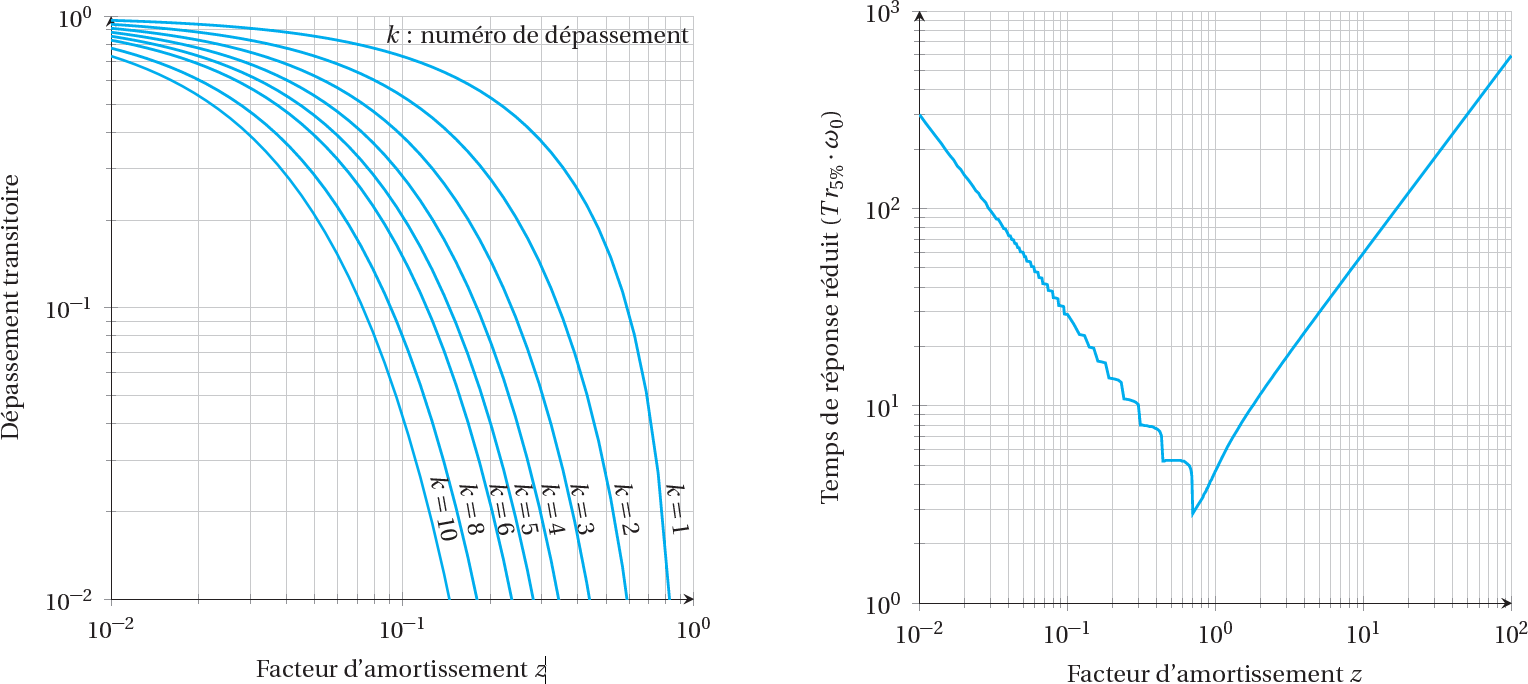
\includegraphics[width=\linewidth]{images/Sujet/images/img_03}
	%\includegraphics[width=.6\linewidth]{images2/identification_BF}

%	\textit{Déplacement de l'instrument en mm.}
	%\label{identification_BF}}
\end{center}


%
%\begin{methode}
%Afin de modéliser le comportement d'un système par une fonction de transfert du deuxième ordre il faut identifier les paramètres $K$, $z$ et $\omega_0$ du modèle $\frac{K}{1+ \frac{2 z}{\omega_0} p + \frac{1}{\omega_0^2} p^2}$:
%\begin{itemize}
%\item $K$: par l'intermédiaire de la valeur finale qui vaut $K e_0$, sachant que $e_0$ est connu;
%
%\item $z$ par le pourcentage de dépassement, grâce à l'abaque des dépassements ou la relation $z=\left( 1+ \frac{k^2 \pi^2}{\ln^2(D_k)} \right)^{-\frac{1}{2}}$;
%\item $\omega_0$ par deux méthodes possibles:
%\begin{itemize}
%\item par le temps de réponse à $5\,\%$ en utilisant les abaques;
%\item par l'instant du premier dépassement, en utilisant l'expression \linebreak $\omega_0=\frac{\pi}{t_1 \sqrt{1-z^2}}$ avec $k=1$.
%\end{itemize}
%\end{itemize}
%
%\end{methode}



\subparagraph{}\textit{Établir, à partir de la courbe de déplacement de l'instrument, l'expression de la fonction de transfert $H_3(p)$ ; déterminer les valeurs caractéristiques : gain statique, coefficient d'amortissement et pulsation propre.}


\subparagraph{}\textit{Déterminer analytiquement la pulsation de coupure à \SI{-3}{dB} pour cette fonction et vérifier si le critère du cahier des charges est respecté.}

\subsection{Analyser le déplacement de l'instrument \\}

La fonction de transfert du système complet est 
$$\frac{1}{(1+\num{0,014} p+\num{0,00017} p^2)(1+\num{0,015} p+\num{0,0014} p^2)}.$$

On donne la courbe d'amplitude (gain) de $H(p)$ pour
$p = j\omega$ dans le plan de Bode.


%%%%% 
\begin{center}
	\includegraphics[width=10cm]{images2/bode_2}

\textit{Diagramme de gain de $H(p)$.}
\end{center}
%\begin{figure}[!h]
%\centering
%\begin{tikzpicture}[xscale=2.8,yscale=1/12]
%\UnitedB
%\OrdBode{10}
%\semilog{-1}{3}{-40}{10}
%\BodeAmp[cyan,thick,samples=100]{-1:2.17}{\SOAmp{1.0}{0.5368754921931593}{76.69649888473704}+\SOAmp{1.0}{0.2004459314343183}{26.72612419124244}}
%\end{tikzpicture}
%\textit{Diagramme de gain de $H(p)$. \label{p04_robot_endo:fig8}}
%\end{figure}
%

La main du chirurgien est prise d'un tremblement sensiblement sinusoïdal dont la période est de \SI{0,25}{s} et l'amplitude \SI{1}{mm}.


\subparagraph{}\textit{Déterminer à partir de cette courbe, l'amplitude du mouvement pris par l'instrument. Quelle est la conséquence de ce mouvement sur la plaie chirurgicale ?}


On souhaite limiter l'amplitude du mouvement de l'outil lors du tremblement de la main en filtrant le signal traité par le capteur -- codeur $C_1$ de sorte que les tremblements n'apparaissent plus sur le soustracteur. On propose trois filtres du premier ordre, de gains statiques égaux à 1 et de constantes de temps : $T_1 =\SI{0,04}{s}$ ; $T_2 = \SI{0,1}{s}$ ; $T_3 = \SI{0,5}{s}$.

\subparagraph{}\textit{Tracer sur le document réponse, les trois diagrammes de gain de ces filtres avec des couleurs différentes.}

\subparagraph{}\textit{Sachant que les mouvements dont la période est inférieure à une seconde ne doivent pas être atténués de plus de \SI{1}{dB},
	indiquer le (ou les) filtre(s) qui ne convient (conviennent) pas.}

Pour filter correctement un tremblement de période \SI{0,25}{s}, il faut compenser le pic de \SI{8,5}{dB}.

\subparagraph{}\textit{Quel est le filtre qui convient le mieux ?}





\subsubsection*{Conclusion  -- Retour sur le cahier des charges}
On donne la courbe d'amplitude corrigée par le filtre le mieux adapté.

\begin{center}
	\includegraphics[width=14cm]{images2/bode_3}

\textit{Diagramme de Bode (gain uniquement) du système corrigé.}
\end{center}

%\begin{figure}[!ht]
%\centering
%{\centering
%%%%% 
%\begin{center}
%\begin{tikzpicture}[xscale=2.8,yscale=1/14]
%\UnitedB
%\OrdBode{10}
%\semilog{-1}{2}{-50}{10}
%\BodeAmp[cyan,thick,samples=100]{-1:2}{\SOAmp{1.0}{0.5368754921931593}{76.69649888473704}+\SOAmp{1.0}{0.2004459314343183}{26.72612419124244}+\POAmp{1.0}{0.1}}
%\end{tikzpicture}
%%\captionof{figure}{Diagramme de Bode (gain uniquement) du système corrigé.  \label{p04_robot_endo:cor3}}\par}
%%\end{figure}
%\textit{Diagramme de Bode (gain uniquement) du système corrigé. }
%\end{center}

\subparagraph{}
\textit{Le critère de bande passante à \SI{-3}{dB} du cahier des charges est-il toujours respecté ?}



\end{document}


\subparagraph{}
\textit{}
\ifprof
\begin{corrige}
\end{corrige}
\else
\fi
